\documentclass[compsoc, conference, a4paper, 10pt, times]{IEEEtran}
\pagestyle{plain}


\usepackage{times}
\usepackage[utf8]{inputenc}
\usepackage{url}
\usepackage{amssymb}
\usepackage{amsmath}
\usepackage{array,multirow}
\usepackage{xspace}
\usepackage{xcolor}
\usepackage{color, colortbl} 
\usepackage{balance}
\usepackage{paralist}
\usepackage{hyperref}
\usepackage{cleveref}
\usepackage{graphicx}
\usepackage{pifont}
\usepackage{array}
\usepackage{booktabs}
\usepackage{tikz}
\usepackage{bm}
%\usepackage{enumitem}%not compatible with IEEEtran it seems
\setlength {\marginparwidth}{2cm}
\usepackage{todonotes}
\usepackage{arydshln}
\usepackage{makecell}
\usepackage{tabularx}
\usepackage{authblk}
\usepackage{caption}
\usepackage{soul,color}
%\usepackage{subcaption}
\usepackage{mwe}
\usepackage{ifthen}
\usepackage{algorithm}
\usepackage[noend]{algpseudocode}
\usepackage{epsfig}
\usepackage[tight,footnotesize]{subfigure}
\usepackage{cite}

\newcommand{\cmark}{\ding{51}}%
\newcommand{\xmark}{\ding{55}}%

%!TEX root = main.tex
%=========================================================

% use true/false to toggle all comments (both kinds)

\newboolean{showcomments}
\setboolean{showcomments}{false}

% ====== comments ======
\newcommand\important[1]{\todo[inline]{\textbf{Important:} #1}}
\newcommand\alberto[1]{\todo[color=yellow,inline]{\textbf{Alberto:} #1}}
\newcommand\etienne[1]{\todo[color=orange,inline]{\textbf{Etienne:} #1}}
\newcommand\pierre[1]{\todo[color=brown,inline]{\textbf{Pierre:} #1}}
\newcommand\felix[1]{\todo[color=blue!40,inline]{\textbf{Felix:} #1}}
\newcommand\michal[1]{\todo[color=green,inline]{\textbf{Michał:} #1}}
\newcommand\onur[1]{\todo[color=red,inline]{\textbf{Onur:} #1}}
\newcommand\sergi[1]{\todo[color=pink,inline]{\textbf{Sergi:} #1}}
\newcommand\ramin[1]{\todo[color=brown,inline]{\textbf{Ramin:} #1}}
\newcommand\mustafa[1]{\todo[color=brown,inline]{\textbf{Mustafa:} #1}}
% Uncomment the following command to make all comments disappear
\ifthenelse{\boolean{showcomments}} { }
{
\renewcommand\important[1]{}
\renewcommand\alberto[1]{}
\renewcommand\mustafa[1]{}
\renewcommand\michal[1]{}
\renewcommand\onur[1]{}
\renewcommand\sergi[1]{}
\renewcommand\etienne[1]{}
\renewcommand\pierre[1]{}
\renewcommand\ramin[1]{}
\renewcommand\felix[1]{}
}

% ====== inlined and toggable comments ======

\ifthenelse{\boolean{showcomments}}
{ \newcommand{\mynote}[3]{
    \protect\fbox{\bfseries\sffamily\scriptsize#1}
    {\small\textsf{\emph{\color{#3}{#2}}}}}}
{ \newcommand{\mynote}[3]{}}

\newcommand{\er}[1]{\mynote{Etienne}{#1}{blue}}
\newcommand{\mk}[1]{\mynote{Michał}{#1}{brown}}
\newcommand{\sr}[1]{\mynote{Sergi}{#1}{red}}

% \newcommand{\xxx}[1]{\mynote{YourName}{#1}{black!20!red!80!}}
% \newcommand{\xxx}[1]{\mynote{YourName}{#1}{green}}
\newcommand{\as}[1]{\mynote{Alberto}{#1}{orange}}
\newcommand{\dk}[1]{\mynote{Daniel}{#1}{green}}
\newcommand{\rs}[1]{\mynote{Ramin}{#1}{violet}}
\newcommand{\oa}[1]{\mynote{Onur}{#1}{red}}

% ====== systems ======
% \newcommand\sysname{TOPDISC\xspace}
\newcommand\sysname{DISCv5\xspace}
\newcommand\discv{DISCv4\xspace}
\newcommand\altname{DHT\xspace}
\newcommand\altnameticket{DHTTicket\xspace}
\newcommand\altsysname{PMETIS\xspace}
\newcommand\sysnamePriv{Pineapple\xspace}
\newcommand\sysnameAnon{\coconut}
\newcommand\libcoin{LibraCoin\xspace}
\newcommand\libcoins{LibraCoins\xspace}
\newcommand\privcoin{PrivCoin\xspace}
\newcommand\privcoins{PrivCoins\xspace}

\newcommand\sysnamereplay{\texttt{byzcuit}\xspace}
\newcommand\sysnamebaseline{\texttt{byzcuit-baseline}\xspace}
\newcommand\simplesysname{Simple-\sysname}

\newcommand\libra{Libra\xspace}
\newcommand\fourier{Fourier\xspace}
\newcommand\chainspace{Chainspace\xspace}
\newcommand\ethereum{Ethereum\xspace}
\newcommand\hyperledger{Hyperledger\xspace}
\newcommand\omniledger{Omniledger\xspace}
\newcommand\rapidchain{RapidChain\xspace}
\newcommand\elgamal{El-Gamal\xspace}
\newcommand\coconut{Coconut\xspace}
\newcommand\macggm{$\bm{\mathrm{MAC_{GGM}}}$\xspace}
\newcommand\sbac{S-BAC\xspace}
\newcommand\bft{BFT\xspace}
\newcommand\atomix{Atomix\xspace}
\newcommand\cscoin{CSCoin\xspace}
\newcommand\rscoin{RSCoin\xspace}
\newcommand\lsbac{\sysname}
\newcommand\fsbac{F-SBAC\xspace}
\newcommand\bftsmart{\textsc{bft-SMaRt}\xspace}

\makeatletter
\def\BState{\State\hskip-\ALG@thistlm}
\makeatother

% ====== custom notations ======
%\newcommand\algorithm[1]{\textsf{#1}}
\newcommand\hashtopoint{H^*\xspace}
\newcommand\stringtopoint{H'\xspace}
\newcommand\function[1]{\ding{118}\xspace \textsf{#1}:\xspace}
\newcommand\shard[1]{\emph{shard}\xspace#1\xspace}
\newcommand\Shard[1]{\emph{Shard}\xspace#1\xspace}
\newcommand\preacceptt{\textsf{pre-accept}($T$)\xspace}
\newcommand\preabortt{\textsf{pre-abort}($T$)\xspace}
\newcommand\preaccepttt{\textsf{pre-accept}($T'$)\xspace}
\newcommand\preaborttt{\textsf{pre-abort}($T'$)\xspace}
\newcommand\preacceptttt{\textsf{pre-accept}($T''$)\xspace}
\newcommand\preacceptts{\textsf{pre-accept}($T,s_T$)\xspace}
\newcommand\preabortts{\textsf{pre-abort}($T,s_T$)\xspace}
\newcommand\preabortttt{\textsf{pre-abort}($T''$)\xspace}
\newcommand\acceptt{\textsf{accept}($T$)\xspace}
\newcommand\abortt{\textsf{abort}($T$)\xspace}
\newcommand\accepttt{\textsf{accept}($T'$)\xspace}
\newcommand\aborttt{\textsf{abort}($T'$)\xspace}
\newcommand\acceptttt{\textsf{accept}($T''$)\xspace}
\newcommand\abortttt{\textsf{abort}($T''$)\xspace}
\newcommand\acceptts{\textsf{accept}($T,s_T$)\xspace}
\newcommand\abortts{\textsf{abort}($T,s_T$)\xspace}
\newcommand\myrow[1]{row\xspace\textsf{#1}\xspace}
\newcommand\mycolumn[1]{column\xspace\textsf{#1}\xspace}
\newcommand\shardled{shard-led\xspace}
\newcommand\Shardled{Shard-led\xspace}
\newcommand\clientled{client-led\xspace}
\newcommand\Clientled{Client-led\xspace}
\newcommand\activeObj{`active'\xspace}
\newcommand\inactiveObj{`inactive'\xspace}
\newcommand\locked{`locked'\xspace}
\newcommand\wa{{WA}\xspace}
\newcommand\wb{{WB}\xspace}
\newcommand\ka{{KA}\xspace}
\newcommand\kb{{KB}\xspace}

% ====== concepts/terminology =======

\newcommand\attacker{attacker\xspace}
\newcommand\adversary{attacker\xspace}
\newcommand\prerecorded{prerecorded\xspace}
\newcommand\prerecords{prerecords\xspace}
\newcommand\prerecord{prerecord\xspace}

%  ===== formatting ======
% Abbreviations etc.
\newcommand{\cf}{cf.\@\xspace}
\newcommand{\vs}{vs.\@\xspace}
\newcommand{\etc}{etc.\@\xspace}
\newcommand{\ala}{ala\@\xspace}
\newcommand{\wrt}{w.r.t.\@\xspace}
\newcommand{\etal}{\textit{et al.}\@\xspace}
\newcommand{\eg}{\textit{e.g.}\@\xspace}
\newcommand{\Eg}{\textit{E.g.}\@\xspace}
\newcommand{\ie}{\textit{i.e.}\@\xspace}
\newcommand{\Ie}{\textit{I.e.}\@\xspace}
\newcommand{\via}{\textit{via}\@\xspace}
\newcommand{\defacto}{\textit{de facto}\@\xspace}

\newcommand\mypara[1]{\vspace{0.05in} \noindent \textbf{#1.}}
\newcommand\para[1]{\vspace{0.05in} \noindent \textbf{#1.}}


\newcommand\definition[2]{\ding{118}\xspace \textsf{#1}\xspace$\bm{\rightarrow}$\xspace(#2):\xspace}



% For inlined section titles.
\newcommand\inlinesection[1]{{\bf #1.}}

\def\first{({\it i})\xspace}
\def\second{({\it ii})\xspace}
\def\third{({\it iii})\xspace}
\def\fourth{({\it iv})\xspace}
\def\fifth{({\it v})\xspace}
\def\sixth{({\it vi})\xspace}

\newcommand{\one}{({\em i})\xspace}
\newcommand{\two}{({\em ii})\xspace}
\newcommand{\three}{({\em iii})\xspace}
\newcommand{\four}{({\em iv})\xspace}
\newcommand{\five}{({\em v})\xspace}

% Colours
\definecolor{verylightgray}{gray}{0.8}

% Table
\newcolumntype{L}{l<{\hspace{1cm}}}
\newcolumntype{C}{c<{\hspace{1cm}}}
\newcolumntype{D}{c<{\hspace{0.3cm}}}

% Markers
\newcommand\vgap{\vskip 2ex}
\newcommand\marker{\vgap\ding{118}\xspace}

\def\na{--}
\def\unsure{?}
\def\missing{$!$}
\newcommand{\yes}{\ding{51}}
\newcommand{\no}{\ding{55}}
\DeclareRobustCommand\pie[1]{
\tikz[every node/.style={inner sep=0,outer sep=0, scale=1.5}]{
\node[minimum size=1.5ex] at (0,-1.5ex) {}; 
 \draw[fill=white] (0,-1.5ex) circle (0.75ex); \draw[fill=black] (0.75ex,-1.5ex) arc (0:#1:0.75ex); 
}
}
\def\L{\pie{0}} % Low
\def\M{\pie{-180}} % Medium
\def\H{\pie{360}} % High


\begin{document}

\title{Topic-based service discovery for the Ethereum P2P network}
\title{\sysname: Service discovery for the Ethereum platform}
\title{Robust service discovery in the Ethereum ecosystem with \sysname}
\title{\sysname: Robust Service Discovery in the Ethereum Ecosystem}
\author{Anonymous submission \#48}
\maketitle
    % \vspace{-0.90in}
\begin{abstract}

The Ethereum ecosystem hosts a steadily increasing number of decentralized applications, including but not limited to the blockchain of the same name. Nodes joining the ecosystem connect to a global peer-to-peer network in which they have to find their application-specific peers. The peer discovery process is crucial for the efficiency and security of the entire ecosystem. Unfortunately, \discv, the current discovery protocol of the Ethereum global network scales poorly with increasing numbers of applications and nodes.

We present \sysname, a novel service discovery protocol for the Ethereum global network. \sysname combines pseudo-random and deterministic placement of advertisements to achieve both efficiency and security. It implements a new admission control protocol that protects against a wide range of malicious behaviors expected in an open environment. 
We implement \sysname in the official Go Ethereum client (geth) and in a dedicated scalable simulator.
In comparison with \discv, \sysname performs lookup operations send up to three orders of magnitude less messages, and discovers ten time more peers per time slot while achieving a similar or lower eclipse probability. 
\sysname is scheduled for deployment in future versions of the Ethereum platform.
\end{abstract}

%!TEX root = ../main.tex
%=========================================================

\er{General comments (20220914) after NDSS reject:
\begin{itemize}
	\item We need to clarify the difference, if any, between \sysname and discv5. Ideally we will want to update the online description which is already several months, if not years, old. I would advocate to present \sysname as the central component of discv5, and detail what are the helping protocols around it (unless, of course, my understanding is incorrect).
	\item Need experiments on prototype.
	\item The use of 100 IPs for the Sybils did not convince one of the two reviewers. Not sure how to fix this?
	\item We should make sure the disctinction between the Ethereum blockchain and the Ethereum ecosystem is clear (confusion with second reviewer).
\end{itemize}
}

\section{Introduction}
With an average of 23,500 constantly live nodes~\cite{discv4-dns-lists}, Ethereum is one of the largest decentralized platforms currently in operation.
While it is widely known for supporting the blockchain of the same name (also known as the \emph{mainnet}), the Ethereum platform is also home to a number of additional decentralized applications.
This includes blockchains used for test purposes (\emph{Ropsten}, \emph{G\"orli}), divergent blockchains resulting from a past fork (\emph{Ethereum classic}), alternative cryptocurrencies (\emph{Pirl}, \emph{Musicoin}), exchange markets (\emph{Binance}), content delivery networks (\emph{Swarm}), or messaging applications (\emph{Whisper}).
The platform already features almost 500 applications, and their number grows every year~\cite{discv4-dns-lists}. The size distribution of the application-specific sub-networks varies significantly (\Cref{fig:ecosystem}) featuring a \emph{long tail}, with a vast majority of applications formed of a few hundred nodes or less.

\begin{figure}[t]
    
\includegraphics[width=1\linewidth]{img/ecosystem}
    \vspace{-0.15in}
    \caption{Distribution of the number of nodes in Ethereum's sub-networks, corresponding to different applications (May 2022).
    Sub-networks are sorted by decreasing popularity.
    A Zipf distribution is given for reference.
    }
    \vspace{-0.20in}
    \label{fig:ecosystem}
\end{figure}

All nodes in the Ethereum platform participate in a \emph{global} peer-to-peer (P2P) network operating a distributed hash table (DHT)~\cite{maymounkov2002kademlia}.
In addition to joining the global network, every node connects to at least one \emph{sub-network} formed of peers participating in its application(s) of interest.
In this paper, we focus on the \emph{service discovery} mechanism, by which a node participating in the global P2P network discovers an application sub-network.
This mechanism returns a set of peers that are used as entry points to the P2P overlay specific to that application, as illustrated by \Cref{fig:subnetwork}.

\begin{figure}[b!]
    \includegraphics[width=1\linewidth]{img/subnetwork}
    \vspace{-0.15in}
    \caption{Formation of application-specific sub-networks using a universal service discovery network.
    }
    \label{fig:subnetwork}
    \vspace{-0.15in}
\end{figure}

Service discovery is a particularly sensitive mechanism in the Ethereum platform.
It must ensure that malicious participants to this open network are unable to bias its execution against a victim node or sub-network--and that, despite the ability of these adversaries to operate multiple Sybil identities.
Of particular importance is the protection against \emph{eclipse} attacks, where an adversary would lure its victim(s) into a sub-network formed of only nodes under its control.
Similarly, an adversary may run \emph{denial-of-service} attacks against a specific application, preventing other nodes from discovering peers from the associated sub-network.
On the other hand, the mechanism must remain efficient and scalable.
It is not desirable, in particular, that it relies solely on a fixed set of dedicated registrar nodes maintaining the membership of each application, both for scalability and robustness reasons. Registrar nodes for popular applications could quickly become overwhelmed, and be an easy target for attackers.
In addition, the need to provision dedicated registrar nodes would be a hindrance to the emergence of new applications and (initially) small sub-networks.

\er{There are inconsistencies with the presentation of discv4; here presented as a set of protocols but later as the name of the discovery mechanism itself. In general, we should clarify what are these other protocols. If these are helping/lower level protocols for the discovery mechanism I would prefer to present discv4 as the discovery mechanism (and do the same for discv5=\sysname).}
The current service discovery mechanism used in the Ethereum platform is part of \discv~\cite{discv4}, a set of protocols leveraging the global DHT.
It employs a simple but robust \emph{random walk} approach.
A node willing to join an application's sub-network simply contacts individually a series of nodes collected from random lookups on the DHT, repeatedly checking application membership until it has collected enough peers participating in this target application.
This approach offers good resilience to malicious behaviors but it suffers from very poor scalability and performance, in particular for small sub-networks. \er{add a sentence or two explaining why it is inefficient for small sub-networks, one reviewer did not get it.}
As more applications join the DHT, the inefficiency of the random discovery process becomes a bottleneck for the entire ecosystem. While alternative solutions for service discovery have been proposed, they are meant for small-scale network~\cite{zhang2002aggregate, helal2002standards}, centralised~\cite{RFC6763}, based on unrealistic assumptions~\cite{danezis2005sybil, danezis2009sybilinfer} or insecure~\cite{baldoni2007tera,scribe,poldercast,banno2015,scribe}. We provide an extensive analysis of these systems in \Cref{sec:related}.

\smallskip
\noindent
\textbf{Contributions.}
%
We detail in this paper \sysname, a novel service discovery mechanism for large-scale, decentralized platforms and its application to Ethereum.
\sysname targets a balance between robustness, i.e., the ability to resist malicious behaviors and Sybil identities, efficiency, i.e., fast service discovery even for small applications, and good load-balance over participating nodes.

After providing background knowledge and reviewing the current service discovery mechanism of Ethereum in \Cref{sec:background}, and detailing our system and threat models in \Cref{sec:model}, we detail \sysname as follows.

In \Cref{sec:placement}, we present how this new protocol enables nodes, members of application sub-networks, to \emph{advertise} their membership to these applications in the form of \emph{service advertisements}.
Any node can act as a \emph{registrar} and store advertisements for any topic.
In contrast with the direct use of the DHT as a key-value store, however, in \sysname service advertisements propagate to a pseudo-random subset of all nodes in the global network.
The density of advertisements for an application increases as a DHT lookup approaches its associated key in the DHT overlay structure.

Robustness, load balancing, and efficiency for the discovery of smaller sub-networks all rely on a novel \emph{admission protocol}, by which registrars accept or reject incoming service advertisements (\Cref{sec:admission}).
It ensures that advertisers cannot effectively flood advertisements at a registrar, even when deviating from the protocol or operating Sybils, and that less popular topics get a sufficiently high probability to be represented and looked up.

At the core of our novel admission protocol lies the need for registrants to respect a waiting time imposed by the registrars before being able to successfully register their advertisement.
We discuss the design and dynamics of the waiting function in \Cref{sec:waitingTime}.
The function allows limiting the amount of resources used by each node, promotes diversity of topic advertisements stored by each node, and protects against a vast range of malicious behaviors.

\er{The relation between discv5 and \sysname is unclear. If discv5 is a set of protocols as written below we should detail what the other protocols are. From the webpage description it seems more that the discovery mechanism is the central protocol and other protocols are helper/subsidiary protocols, e.g., for defining the communication standards between nodes in the p2p operation. We should make it clearer that \sysname is the core component of discv5 (or even consider using discv5 name directly if possible, and mention that the other protocols are helpers, if the reasoning above applies).}
We overcome multiple practical challenges, implement \sysname in a simulator as well as in the code base of \emph{discv5}~\cite{discv5} (\ie, Node Discovery protocol version 5) - a new set of P2P protocols replacing \emph{discv4}~\cite{discv4}. 
%We intend to release the full code and dataset of our experiment open source with the unblinded version of this paper.
Compared to the current Ethereum discovery protocol, \sysname discovers 10 times more peers on average by sending two times less lookup messages and achieves a similar or better resistance against eclipse attacks. Compared to vanilla DHT operations, our system reduces load on the most busy node in the network by 2 orders of magnitude and is up to 4 orders of magnitude less likely to be eclipsed by a powerful attacker. \er{the metric for the ``eclipsability'' here is not clear. What does it mean to be 4 OOM less likely to be eclipsed?}
\sysname is currently under testnet evaluation and is scheduled for deployment in the future versions of Ethereum network. \er{revise previous if the deployment is actually planned.}


\section{Background}\label{sec:background}
\michal{Need a good introduction on Kademlia here. Distances/buckets etc. It's required to explain the ticket table, routing etc.}

%!TEX root = ../main.tex
%=========================================================

\section{System and threat models}
\label{sec:model}

\begin{table}
    \caption{Notation}
    \label{tab:notation}
\begin{center}
    \begin{tabular}{ | l | p{8cm} |}
      \hline
        $N$ & network size \hl{Consider changing to all nodes so that $n \in N$} \\ \hline
        $k$ & number of peers holding a key in the DHT (from the background section) \hl{not sure we need it - it's only in the background and we can explain everything by finding just 1 closest peer to the key} \\ \hline
        $X$ & a node (from the background section) \\ \hline
        $n$ & \hl{a node (from the 4.1)} \\ \hline
        $n$ & total size of the ad cache (Sec. 5.2) \hl{a clash with node} \\ \hline
        $p$ & peer (section 4.1) \\ \hline
        $T$ & Table (section 4.1) \\ \hline
        $b_i$& $i$-th bucket (section 4.1) \hl{TODO: add key} \\ \hline
        $\alpha$ & number of concurrent routing operations \\ \hline
        $K_{\textit{register}}$ & number of ads placed per bucket\\ \hline
        $K_{\textit{lookup}}$ & \hl{It's weirdly defined in Sec. 4.4}: search process progresses using maximum $K_{\textit{lookup}}$  parallel requests, and issuing requests towards up to $K_{\textit{lookup}}$  peers per bucket.\\ \hline
        $a$ & ad lifetime  (Sec. 4.3)\\ \hline
        $N_{\textit{lookup}}$ & number of peers to find (Sec. 4.4) - \hl{could be introduced before specifying what the system does} \\ \hline
        $N_{\textit{return}}$ & max number of topic-specific peers returned from a single registrar \\ \hline
        $t_{\textit{init}}$ & ticket: the local time at the registrar when the ad was received for the first time \\ \hline
        $t_{\textit{waiting}}$ & ticket the local time at the registrar when the ad was received for the first time \\ \hline
        $\delta t_{\textit{window}}$ & registration window \hl{we probably don't need both $\delta$ and "window"} \\ \hline
        $t_{\textit{cumulative}}$ & ticket:cumulative waiting time \\ \hline
      \hline
    \end{tabular}
  \end{center}
\end{table}
\mk{TODO: add notation for number of malicious nodes, number of malicious IPs etc.,}
\mk{change bucket definition to add the target key (can be useful to define advertise tables etc. if we introduce them in the background \eg $b_i(key)$). We also often indicate the farthest buckets - we could simply use $b_0$}
\mk{Put macros for the notation}
\mk{We need a notation for an ad - at the end of Sec. 5.2 we just use "Ad".}


In this section, we present our network and threat models as well as the target properties of \sysname. 

\subsection{System model}

We assume a network of $N$ nodes.\footnote{$N$ is unknown to the participants but is used in our analysis.}
At startup time, each node generates a public/secret key pair, which it uses to secure point-to-point communication with its peers.
Nodes are identified by their \emph{node ID}, which is simply the hash of their public key.
Multiple nodes may share the same IP address (due to NAT or being hosted by the same physical machine)~\cite{marcus2018low}.
However, two nodes cannot share the same ID.

% \er{revise: It is not clear \sysname is an extension of discv5 from the online documentation, but rather its central mechanism. What are the other protocols as part of discv5  is also unclear.}
% \sysname is built on the existing Ethereum DHT. Specifically, we designed and implemented our system as an extension of Ethereum's \emph{Node Discovery Protocol v5 (discv5)}. However, the operation of service discovery is not Ethereum-specific and could also be implemented using a different DHT. \er{I would not necessarily make this claim here, since several operations are. Kademlia-specific in reality. Maybe save for the conclusion?}

As for \discv, \sysname leverages the existing Ethereum DHT, but does not rely on its key lookup operations.
\sysname indexes different applications in the Ethereum eco-system as \emph{topics}.
A topic is an identifier for an application, or \emph{service}, provided by a node.
Topics are arbitrary strings that hash to a specific key. % in the DHT key space.

All DHT nodes fulfill the following roles:
\begin{itemize}
    \item A \textbf{registrar} accepts advertisements (\emph{ads}) and responds to topic queries. 
    When asked for a specific topic, a registrar responds with nodes that registered ads for this topic.
    % All DHT nodes act as registrars. 
    A registrar may accept and store ads for any topic.
    \item An \textbf{advertiser} registers for a specific service topic and wants to be discovered by its peers.
    Advertisers make themselves discoverable by placing ads for that topic.
    Nodes are advertisers for every service they participate in.
    \item A \textbf{searcher} attempts to discover nodes registered under a specific topic, using service lookup operations.
\end{itemize}

A node providing a certain service topic is said to \emph{register} itself when it submits an ad to a registrar. % to make itself discoverable under that topic.
Depending on the needs of the application, a node can advertise multiple topics or no topics at all. 
We assume that the popularity of topics in the system is highly heterogeneous, i.e., it can follow a power law distribution~\cite{kim2018measuring}.
Anyone can participate in registering and searching for (one or more) topics and use the same ID and IP for all its topics. 

\subsection{Threat Model}
\label{sec:threat}

\sysname is designed to operate in an open, adversarial environment.
We assume the presence of malicious actors in the network that may arbitrarily deviate from the protocol and coordinate their actions.
Malicious actors can spawn multiple virtual nodes within one physical machine, and operate multiple physical machines.
As a result, they can control a number of Sybil node IDs.

% \er{should we mention collusions here? It is mentioned only at the end of the section (although we do not seem to consider it so much in the experiments)}\mk{In the experiments we assume that all the Sybils ae controlled by a single entity. I've expanded the phrase above. I hope it's fine now.}
% % These actors do not strictly follow the protocol when communicating with others and attempt to influence the discovery results of honest nodes by steering them toward the attacker-controlled nodes.

The security of the service discovery mechanism is fundamentally dependent on the security guarantees provided by the underlying DHT implementation, and in particular on its ability to avoid eclipse attacks against a specific node.
Indeed, even if \sysname does not rely on DHT lookup operations, information in the DHT routing table is used to initialize and maintain the data structures used by the service discovery layer.
We assume, therefore, that no honest node is fully eclipsed by the malicious ones, \ie, each honest DHT node has \emph{at least} one honest peer.
As previously mentioned, Ethereum already implements multiple mechanisms preventing eclipse attacks at the DHT level~\cite{marcus2018low, henningsen2019eclipsing}.  

Maintaining nodes in the DHT requires infrastructure resources (public IP addresses) and we assume that the resources under the control of an attacker are limited.
Specifically, we assume that it is easier for an attacker to generate similar IP addresses (\ie within a single subnet) than it is to control many diverse IP addresses (with different prefixes).
We use the number of IP addresses and IDs under the control of an attacker as parameters for our evaluation in \Cref{sec:eval}.

\mk{We can probably remove those and mention those problems when introducing our system.}
Through a literature review~\cite{chen2020survey, henningsen2019eclipsing} we collected a list of malicious behaviors that an attacker can use to disrupt a DHT-based service discovery protocol:
\begin{itemize}
    \item \textbf{Malicious DHT Peer}: DHT routing relies on asking peers for other nodes, closer to a specific target. When responding to such requests, an attacker only returns other malicious nodes, in order to hijack the process of DHT traversal by honest nodes. \er{this seems contradictory with the fact that we wrote two paragraphs ago that we assumed the DHT to be secured against Sybils. Should we change DHT routing to something more generic, like an exploration process?} \er{also, this may appear contradictory to the fact we do not use the DHT routing (lookup) directly but implement our own}
    \item \textbf{Malicious Registrar}: When queried for a specific topic, an attacker returns a maximum amount of malicious nodes.\footnote{Alternatively, a malicious registrar could simply refuse to respond. However, such behavior is less effective than returning malicious peers.}
    \item \textbf{Spamming Advertisers}: An attacker bombards honest registrars with malicious ads. The attack can target single or multiple topics. The attack may cause an honest registrar to refuse honest ads due to lack of resources (\eg, storage and CPU power). This registrar will, furthermore, later return maliciously-inserted ads of the spammer when queried by honest searchers. 
    \item \textbf{Generic Spammers}: An attacker bombards an honest registrar with topic queries or random traffic hoping to exhaust bandwidth or CPU power.
\end{itemize}

Adversaries can strategically target specific nodes or regions in the DHT key space (\ie by generating Sybil Node IDs within the desired region) when implementing these attacks.
We assume the presence of attackers that can combine some or all of the behaviors above, and coordinate their actions to maximize their effect. 

\subsection{Target Properties}

Under the considered threat model, \sysname achieves the following properties.

\para{Efficiency} 
\sysname ensures that the number of nodes contacted and the number of messages exchanged increase logarithmically with the number of system participants, for both lookup and register operations. 
Sending and processing service discovery requests requires only simple operations involving a constant amount of resources.
The storage usage for the registrars is limited by a configurable but fixed cap that does not depend on the amount of incoming traffic. 

\para{Fairness}
\sysname ensures a balanced load distribution across systems participants and regions of the key space (\ie, it avoids \emph{hotspots}).
The system provides efficient lookup and registration operations for all participants regardless of the topic they look up or register for.
Each advertiser has a similar probability of being discovered by its peers. 
% \er{we should ideally be a bit more formal here and give bounds (in big O?) of the unbalance between these nodes.}\mk{What fairness metric would you suggest here?} \er{this would be ratio between the likelihood of being discovered for a popular and a less-popular advertiser}

\para{Security}
\sysname focuses specifically on preventing \emph{Denial of Service} (nodes are unable/slow to discover their application-specific peers) and \emph{Eclipse} (nodes discover uniquely malicious nodes) attacks.
While completely eliminating such attacks in an open network is technically impossible, \sysname provides high probabilistic security 
% \er{can we quantify this probability?}\mk{It depends on a lot of factors \#Sybil, \#malicious\_IPs etc. so not easy, but I'll think about it.} \er{commenting for now, no time}
and increases the monetary cost of committing them. 
% under the presence of a powerful attacker.


%!TEX root = ../main.tex
%=========================================================

\section{Ads placement}
\label{sec:design}
In the following, we provide a description of distributing advertisement in the network and discuss the process of search and establishing sub-protocol connections. 


\subsection{Data Structures}
We start by describing data structures necessary for topic-specific registrations and lookups. 

\para{Registration Table}
In order to execute the ad distribution process described below,  each advertiser maintains a per-topic \emph{registration table} for each advertised topic. The table keeps track of the ongoing registration attempts with different registrars.  The registration table is similar to the routing table used in Kademlia protocol (as described in \Cref{sec:background}). It stores advertiser's peers divided into k-buckets. However, instead of placing nodes in buckets based on the distance from the advertiser, it uses the distance from the topic ID. I.e. the registration table stores $k$ potential registrars for every distance range (bucket) from the topic ID (\Cref{fig:ticket_table}). When created, the table is initialized with peers from the routing table. 

\begin{figure}
    
\includegraphics[width=0.45\textwidth]{img/ticket_table}
    \caption{Creation of ticket table from the routing table.}
    \label{fig:ticket_table}
 \end{figure}

\para{Search Table}
The ad lookup process is supported by a \emph{search table}. 
Searchers maintain a separate table per topic they are currently looking for. 
\ie for each topic the client wants to start discovering nodes, a new \emph{search table} is created. 
Similar to the \emph{registration table}, the \emph{search table} also stores k-buckets of registrar nodes by distance to the topic hash and buckets are initially filled from the local routing table organised by the distance from the topic hash.

%and a new 'search table' is created for each topic. 
%The bucket size \texttt{k}  of the search table should be relatively large in order to make the search efficient. 
%By default we use\texttt{k=16},  similarly to the local routing table (Kademlia DHT).
%Tickets are not required for search and nodes can not be added multiple times in the same k-bucket.

\subsection{Distributing ads across registrars}\label{sec:registration_multi}
When an advertiser wants to associate themselves with a topic, they start by creating a topic-specific \emph{registration table} (as described above). 
Every peer present in the registration table is a potential registrar. 
The objective of the ad placement process is to continuously maintain $K$ active (\ie unexpired) registrations in every bucket. 
Buckets located close to the topic hash cover less hash space than buckets located further away and, in turn, contain less potential registrars. 
Placing a fixed amount of ads per bucket, make registrars close to a topic hash more likely to receive registrations for that specific topic. 
Increasing $K$, makes the advertiser easier to find at the cost of increased communication overhead. 


The advertiser starts by the first bucket (the furthest away from the topic hash) in the \emph{registration table}, selects $K$ random peers and attempts to perform a registration. 
We describe details on the registration procedure in \Cref{sec:registration_single}. 
A successful registration places an ad on an advertiser for a fixed amount of time $t_\textit{lifetime}$.
If a registration is unsuccessful (the selected registrar is down or refuses to store the ad), the advertiser selects another random peer from the same bucket and retries the registration process. 
The advertisers always maintains $K$ attempts and/or successful registrations per bucket unless less than $K$ peers are present in a specific bucket. 
The advertiser repeats the process for every bucket in the registration table. 
\michal{An algorithm here?}

As mentioned above, the \emph{routing table} is initialized with the peers already present in the routing table. It is thus possible that an advertiser will not know any nodes in buckets located close to the topic hash\footnote{This usually happens when the advertiser's ID is distant from the topic hash.}. 
To fill the empty buckets, the advertiser asks potential registrars to return $N$ closest peers to the topic hash they know of. 
The procedure is similar to the regular DHT \emph{FIND\_NODE} operation described in \Cref{sec:background}. 
The registrars respond with a list peers regardless of the success of the registration operation. 
The advertiser uses the returned information to populate its \emph{registration table}. 
As the advertiser progresses through the buckets, it queries potential registrars located closer to the topic hash and thus having a more detailed view of this part of the network. 
Similarly to the DHT routing, the registration procedure is guaranteed to find the closest node to the topic hash in the network. 



%In addition to that, every time a node sends a ticket or registration request, the registrar replies with the closest nodes to 'the topic hash' that it knows. 
%This helps filling up k-buckets without sending additional lookups. 
%Also, when performing topic search (sending lookups for specific topics),  closest known nodes to 'the topic hash' are attached by the registrar node in the response.




\subsection{Topic Search}\label{sec:lookup}
To find ads, \sysname uses a process similar to the registration procedure. 
The goal is to find $N_\textit{lookup}$ node advertised with a specific topic. 
The searcher starts by creating a topic-specific \emph{search table} initially populated with nodes from the \emph{routing table}. 
\michal{Should we have separate $K$ for registration and lookup? You might argue that if less ads are placed, more lookups are needed and vice-versa.}
The searchers progressively moves through buckets (starting from the furthest away), randomly chooses $K$ registrars per buckets and sends them lookup requests. 
Each queried registrar responds with a list of $N_\textit{return}$ topic-specific advertisers the registrar know of. If the total number of topic-specific registrations is larger then $N_\textit{return}$, the registrar return a random subset. While both $N_\textit{return}$ and $N_\textit{lookup}$ are protocol parameters, the amount of ads returned by a single registrar must be lower than the total number of ads searchers are aiming to find $N_\textit{return} < N_\textit{lookup}$. It allows to diversify sources of ads received by the searcher. I.e., a single malicious registrar is not able to stop an honest searchers from contacting other nodes.
There is a tradeoff between overhead and security when choosing $N_\textit{return}$ and $N_\textit{lookup}$. 
By requiring a large amount of total ads to stop the search ($N_\textit{lookup}$) and low amount of ads returned by registrar $N_\textit{return}$ a higher diversity of data sources is achieved by the cost of contacting a large number of registrars. On the other hand, similar values of both $N_\textit{lookup}$ and $N_\textit{return}$ reduce the overhead but increase the danger of a searcher receiving ads uniquely from malicious nodes. Finally, low values of $N_\textit{lookup}$ stop the search operation early, before reaching registrars close to the topic hash, contributing to more equal load spread. We investigate the impact of both parameters in \Cref{sec:eval}. 
Once ads are discovered, the searcher initiates topic-specific connections based on resules specified by the application. 





\subsubsection{Updating connections}
\michal{Didn't touch this subsection. Should it be here?}
Using the search results, a searcher updates its subprotocol-specific connections. 
For instance,  each Ethereum client keeps connections towards 50 other nodes,  2/3 of those are for inbound connections (\ie 34 connections) where the client has no control over them, and the rest (about 16 connections) are four the outbound connections initiated towards the discovered nodes using the discovery protocol. 
When a lookup is done,  the nodes discovered are stored in a buffer. 
For each node of the buffer a connection is initiated. 
The connection can be successful when the node targeted is alive and has empty slots in the inbound connections,  otherwise the connection is unsuccessful and a new node is selected.
The nodes from the buffer are consumed as connections are attempted to the nodes.
The buffer not only stores the nodes information but also the registrar node that replied with it.
In order to avoid eclipse attacks it is recommended not to start connections with nodes coming from the same registrar. 
Therefore connections are initiated always trying to keep the maximum diversity of the  registrars nodes used.

%\onur{need to explain this process since security depends on that.}

%All the modifiers from the first part of the equation increase with increasing number of the same items that are already in the table, i.e., reduction in diversity. Thus it's getting increasingly difficult to register ads for the same IP/ID/topic. For instance, ads for less popular topic will receive lower waiting times than popular ones. Note that the table does not prevent anyone from registering, but rather makes it slower for already popular items. Such a mechanism promotes diversity in the table and protects against Sybil attacks so that an attacker who is in control of a limited pool of IP addresses won't be able to dominate the table with many ads. The low exponent for the topics is motivated by the topics in the network that are likely to follow a skewed (e.g., a zipf-like) distribution. In contrast, honest nodes' IPs/IDs should follow a uniform distribution.

%The latter part of the formula is determined based on a multiple of ad-lifetime and the current utilisation (i.e., occupancy divided by capacity) of the table. When the utilisation becomes closer to 1.0, the base time becomes very large due to a very small denominator. Before the waiting time becomes infinite (when utilisation becomes 1), the waiting time becomes extremely high, in which case the advertisers give up as explained in the ad distribution process.

%The advertiser attempts to place an ad on each registrar and keeps the latest ticket issued by that registrar. It also keeps references to all pending tickets in a priority queue keyed by the expiry time of the ticket so it can efficiently access the next ticket for which a placement attempt is due.
%Since the table is limited to K values per bucket,  this means there are K on-going registrations per distance to the topic hash id. 
%The number of buckets used in the ticket table is a configurable parameter, but it is recommended to use small number of buckets,  instead of using a bucket per bit of the address space,  to avoid overloading registrars with IDs close to the topic hash. 
%Any node with a distance below the maximum distance minus the number of buckets will be stored in the same bucket.
%In our evaluation we used a ticket table with 10 buckets. 



%This objective is achieved by the advertisers setting a timer with a duration of ad-lifetime immediately upon the receipt of a REGCONFIRMATION from a node in a bucket b, and once the timer expires (after ad-lifetime passes) the advertiser starts a fresh registration with a node that is also located in bucket b. 
%The ticket table is used to store the tickets obtained for each on-going registrations and to keep track of the expiration times of active registrations.

%\subsubsection{Bucket refresh}

%The Ticket table needs to be initialised and refreshed to fill up all the per-distance k-buckets. 
%Ideally,  all k-buckets should be constantly full,  meaning that the advertisers place registrations at registrars in all distances to the topic hash. 
%An option to fill up all k-buckets would be to send periodic lookups for the specific distance to the topic hash, but since there are some distances that tend to be empty in the id space,  sending periodic lookups for the topic hash may create an additional overhead that can be too expensive and create too much traffic in the network. To avoid that, initially, the 'ticket table' k-buckets are filled performing local Ethereum routing table lookups to all distances to the 'topic hash' of the advertised topic.


%\michal{The below seems like an implementation detail.}
%There is  also a refresh bucket process,  similar to the Kademlia DHT table,  where periodically a random bucket is checked to see if it is empty.
%The \texttt{refresh time} is a configurable parameter. 
%We set a \texttt{refresh time=10 seconds} as a reference for our performance evaluation.
%During the refresh process,  in case the bucket checked is empty, 
%a local lookup to the Kademlia DHT table is performed. 
%In case no nodes have been found for the bucket distance,  a Kademlia lookup is performed towards the topic hash~\footnote{The lookup is performed by sending a FINDNODE message,  as described inhttps://github.com/ethereum/devp2p/blob/master/discv4.md.}
%Also, all nodes in the checked bucket are pinged to check they are still alive. 
%In case they are not, tickets for those dead nodes are removed from the ticket table and registrations to new nodes are initiated.




%We implemented and evaluated a lookup strategy that choose which nodes from which buckets ask first trying to diversify the nodes discovered as much as possible and trying not to overload nodes close the topic hash.
%A random node is picked from a bucket following a round-robin approach. 
%It starts picking a random node from the highest distance bucket and follows to the next distance in the bucket list.
%In order to find new results,  bucket entries are replaced when the node fails to answer or when it answers with an empty list of ads. 

%There is also a refresh process,  equivalent to the \emph{ticket table} refresh process, where random buckets are selected and all nodes in the buckets are checked for liveness.
%In case the bucket is empty a Kademlia lookup is performed towards the topic hash.

%!TEX root = ../main.tex

\section{Admission Protocol}\label{sec:admission}
In this section, we describe a registration procedure followed by an advertiser to place an ad on a specific registrar.

\subsection{Challenge}
Registrars have a limited amount of memory and can store only a finite number of ads. If the registration demand surpasses the supply each registrar has to decide which ads should be admitted. In an open setting, implementing simple replacement policies such as Least Recently Used (LRU) or Most recently used (MRU) exposes the system to an attacker that bombards registrars with dummy ads and evicts honest ones.

\mk{TODO:Mention previous work suggested by the NDSS reviewers~\cite{liu2010netfence, crowcroft2007lazy, kung2015practical}}

\sysname solves this problem by using a lightweight \textit{waiting-time-based admission mechanism} for access control. When an advertiser sends an ad placement request to a registrar, the registrar will calculate the amount of time the advertiser needs to wait before being admitted. This \emph{waiting time} is calculated based on the diversity of the request (\ie how different is the request from ads already in the registry) and the space left in the registry. We explain the waiting time calculations in \Cref{sec:waitingTime}. The advertiser must wait for a waiting time reported by the registrar and only then, its ad will be admitted. \er{maybe write ``before it is allowed to contact the registrar again and have its ad admitted''; or we may understand that the ad is accepted without actiom from the advertiser itself.} 

\subsection{Data Structures}
\para{Advertisement}
When advertisers send a registration request, they send an \emph{advertisement} (\emph{ad} in short). The ad contains the IP address of the advertiser, the ID of the advertiser, the topic the ad is for and additional information needed to later contact the advertiser (\eg an application-specific port number). In the remaining part of the paper, we omit the additional information for brevity. 

\para{Ad cache}
Registrars store received ads locally in a data structure called an \emph{ad cache}. Each ad stored in the ad cache has an associated lifetime, after which the ad is automatically removed. Once an ad is added to the cache, the lifetime is set to a fixed value $a$. The total size of the ad cache is limited by $n$. \sysname does not impose topic/IP/ID-specific limits on the content of the \emph{ad cache} to accommodate for diverse network conditions and application popularity distributions.
A single advertiser may place at most one ad for a specific topic in the ad cache (registration requests for ads already in the cache are ignored).
However, an advertiser may attempt to place ads for multiple topics at the same registrar.

\para{Ticket}
Tickets are immutable objects issued by registrars to advertisers when receiving a registration request. Each ticket contains:
\begin{itemize}
    \item Ad - a copy of a registration request (as described above). 
    \item Initial timestamp - the local time at the registrar when the ad was received for the first time, $t_\textit{init}$
    \item Waiting time - the waiting time calculated by the advertiser for the ad, $t_\textit{waiting}$. We describe the details of the waiting time calculations in \Cref{sec:waitingTime}. 
\end{itemize}
The tickets are digitally signed by the issuing registrar. \er{should we give more details here? What is the purpose? Do we assume the registrar knows the public key of the advertiser, always, so it can check this signature?}\mk{It was actually a mistake (now corrected). The ticket are signed by registrars (not advertisers). The registrars issues the ticket to the advertiser and signs it so that when the advertisers comes back, the registrar can verify the integrity of the ticket. It's kind of explained later, so not sure whether we should include more info here.}

\subsection{Registration Procedure}
An advertiser willing to register an ad at a registrar starts by sending an
initial request uniquely containing the ad itself. Based on the
content of the ad cache and the registration, the registrar calculates an
ad-specific waiting time. The advertiser then issues a ticket including the
calculated waiting time and the time of receiving the initial request and sends it back to the advertiser.

The advertiser waits for the indicated time and attempts to register again. The consecutive registration request must include the last ticket issued by the registrar. Tickets can be used uniquely during a registration window:
\begin{equation}\label{eq:registration_window}
    t_\textit{window} = [t_\textit{init} + t_\textit{waiting}, t_\textit{init} + t_\textit{waiting} + \delta t_\textit{window}]
\end{equation}
All the registration requests outside the registration window are ignored by the advertiser. The registrar calculates the registration windows based on the content of the ticket. $\delta t_\textit{window}$ should be chosen to accommodate for the maximum delay between the advertiser and the registrar. The mechanism prevents an attacker from gathering many tickets, accumulating long waiting times (see below) and submitting the tickets all at once to overwhelm the registrar. 

The advertiser calculates a new waiting time, based on the current content of
the ad cache, every time it receives a registration request (with or without
a ticket). The waiting time in the ticket is used only to calculate the
registration windows and prevent advertisers from trying to register
continuously. The ticket also allows the calculation of an accumulated waiting time:
\begin{equation}
    t_\textit{cumulative} = \textit{now} - t_\textit{init}
\end{equation}
An ad is admitted iff the accumulated waiting time is equal to or larger than the calculated waiting time $t_\textit{cumulative} \ge w$\footnote{Note that a registration request without a ticket may be admitted directly iff the calculated waiting time equals to $w=0$.}. For registration requests without a ticket $t_\textit{cumulative} = 0$. An advertiser that misses its registration window (as specified by the most recent ticket), loses all its cumulative waiting time and must attempt to re-register without a ticket. Once an ad is admitted, the registrar confirms the registration to the advertiser.

If the cumulative time is not sufficient, $t_\textit{accumulated} < t_\textit{waiting}$, the registrar issues a new ticket and the advertiser repeats the whole procedure. With consecutive registration attempts, advertisers increase their cumulative waiting time $t_\textit{cumulative}$ and eventually will be admitted. 


\begin{figure}
    
\includegraphics[width=0.45\textwidth]{img/registration}
    \vspace{-0.15in}
    \caption{Registration operation.}
    \label{fig:registration}
    \vspace{-0.15in}
\end{figure}

The inclusion of issue-time allows the registrars to prioritize advertisers that have been waiting for the longest, as we explain later. The tickets are immutable (i.e., tampering with the ticket is detectable by the registrars that originally issued the ticket). \er{maybe explain how we achieve this.} When a registrar issues a new ticket (in case registration is not immediately successful) to an advertiser, the registrar simply copies the issue-time from the last issued ticket and uses that as the issue-time of the new ticket. This means that the registrars are not required to maintain any state for each ongoing ticket request given that they can verify the authenticity of the ticket in the incoming registration requests.



An advertiser gives up and stops the registration process with a registrar when it has received $r$ unsuccessful registration attempts (i.e., after being issued $r$ tickets without being admitted). In this case, the advertiser removes the registrar from its advertise table and selects a new node located in the same bucket and attempts a new registration procedure. The mechanism prevents malicious registrars from stalling honest advertisers.
%\michal{Is the below true? Shouldn't we try to register at the same node?}
%\sergi{We dont use the same, we pick another randomly. we could use the same but i think for diversity could be better  this way}
Similarly, after the expiration of a previously placed ad, the registrar is removed from the advertise table \er{consistency: sometimes advertise table is in italics, sometimes not. Suggest to use italics only the first time the term is used.}\mk{good idea} and the process is restarted with a new node picked from the local route table.%\footnote{We assume a common expiration time for all the registrar. However, each registrar may choose to implement its own expiration time and communicate it to advertisers in the confirmation message}.


\section{Waiting Time}
\label{sec:waitingTime}

The waiting time function is used to calculate the total time advertisers have to wait before being admitted to the ad cache. 
The function directly shapes the structure of the ad cache,  determines its diversity and performs flow control. 
It also protects against attacks, where a malicious actor tries to dominate the ad cache and exhaust resources of the registrar. 

Each request is given a waiting time based on the IP address of the registrar, the topic of the request and the current state of the ad cache. 
The waiting time function is divided into three parts: \emph{occupancy score} (ranging from $0$ to $\infty$) and  \emph{similarity score} (ranging from $0$ to $2$) and is normalized by the amount of time each ad spent in the cache $a$ (\ie \emph{ad lifetime}). $a$ determines the absolute values of the returned waiting time. The final result is a product of all three: $w = a \times \textit{occupancy score} \times \textit{similarity score}.$

The \emph{occupancy score} is based uniquely on the number of the ads already in the cache.
Its role is to progressively increase the waiting time as the ad cache fills up and to limit the memory used by a registrar.
The \emph{occupancy score} is defined by equation~\ref{eq:occupancy}:

\begin{equation}
\label{eq:occupancy}
    \textit{occupancy score} = \frac{1}{(1-\frac{d}{n})^{P_{occupancy}}}
\end{equation}
where $d$ is the number of ads in the cache, $n$ is the capacity of the cache. $b$ and $P_{occupacy}$ are protocol configurable parameters. 
When the number of ads in the cache is low ($d \ll n$ ), the \emph{occupancy score} goes to $1$. 
As the ad cache fills up, the score will be amplified by the divisor of the equation. 
The higher values of $P_{occupancy}$, the faster the increase. 
With the current occupancy $d$ close to the capacity of the cache $n$, the \emph{occupancy score} goes to infinity thus limiting the number of admitted requests. We analyse the behavior of the waiting function and choose optimal system parameter values in \Cref{sec:analysis}.

The role of the \emph{similarity score} is to determine how similar is the incoming request to the ads already in the ad cache in terms of the IP address and the topic. 
Requests significantly different from the current content of the cache receive lower similarity score resulting in lower overall waiting time. 
Such an approach promotes fairness across topics (it is easier for less popular topics to get into the cache) and protects against attempts to fill the ad cache by a small number of advertisers (as identified by their IP addresses). The similarity score is defined as a sum of similarity score for IP and the topic of the request and a system parameter $b$: $\textit{similarity} = b + \textit{similarity(topic)} + \textit{similarity(IP)}$. 

The system parameter $b$ ensures that the waiting time never reaches $0$ even when requests get $0$ values for IP and topic similarity score. Together with $P_\textit{occupancy}$, it shapes the behaviour of the waiting functions. We choose values for those parameters in \Cref{sec:analysis}.

The similarity score for topics is given by equation~\ref{eq:similarity}:
\begin{equation}
\label{eq:similarity}
    \textit{similarity(topic)}= \frac{d(topic)}{d}
\end{equation}
where $d(topic)$ is the number of ads for the specified topic already in the cache and $d$ is the total number of ads in the cache. 
The score goes to $1$ as the specified topic dominates the cache $d(topic)  \approx  d$. 

%For calculating the IP address diversity \sysname uses a different similarity score. 
A simple similarity score used for topics cannot be securely applied for IP addresses. 
An attacker may be able to generate a large number of different addresses sharing the same prefix (\eg using a single /24 IPv4 network) that, while similar, would receive low \emph{similarity scores}. 
The Go Ethereum client~\cite{geth} limits the number of IP addresses coming from the same (\eg /24 IPv4 address) network.
However, it is impossible to reliably set those limits without knowledge about the network size or NAT configuration of honest nodes. 
Instead, we propose an approach that directly captures the similarity level across different IPs and translates it into a numerical score. 

We introduce a binary \emph{tree}, as shown on \Cref{fig:ip_tree}, that stores IP addresses used in the existing registrations in the ad cache.
Each node stores a counter, while the edges represent consecutive $0$s or $1$s in a binary representation of IP addresses.
For simplicity,  we present the \emph{tree} for IPv4 addresses but its adaptation for IPv6 is straightforward.

\begin{figure}
    
\includegraphics[width=0.45\textwidth]{img/ip_tree}
    \caption{Inserting an IP address into the IP \emph{tree} structure. \mk{TODO:make it up to date, smaller and consistent with other figures.}}
    \label{fig:ip_tree}
\end{figure}

Apart from its root,  the \emph{tree} consists of 32 levels (33 levels in total) representing bits in the binary representation of IPv4 IP addresses. 
The root level is depicted as level $0$, the level of its successor as level $1$ and so on. 
The counter of every \emph{tree} node is initially set to $0$. When adding an IP to the \emph{tree},  the address is first converted to its binary representation and follows a path in the \emph{tree} corresponding to consecutive bits. 
Counters of all the visited nodes are increased by $1$. 
As a result, the root counter stores the number of all the IP addresses in the ad cache, its $0$ successor stores the number of the IP addresses starting with $0$, its $1$ successor stores the number of the IP addresses starting with $1$ and so on. 
Removing an IP from the \emph{tree} follows the analogical procedure but decreases all the counters on the path. 

After each addition of an address to the \emph{tree} a score is generated.
The score is a sum of \emph{penalty points} of obtained on visited nodes. 
$$score(IP)=\sum_{i=1}^{32} \textit{penalty}(p_{\geq i}) $$
where $p_{\geq i}$ is the number of IP addresses in the cache sharing a prefix with $IP$ with a length of at least $i$. A penalty point is given at $p_{\geq i}$ if the IP address to be added makes the tree more unbalanced than the tree currently is:

\begin{equation}
    \textit{penalty}(p_{\geq i})=
    \begin{cases}
      0, & \text{if}\ p_{\geq i} \leq \frac{p_0}{2^i} \\
      1, & \text{otherwise}
    \end{cases}
  \end{equation}

The counter values are taken \emph{before} the increment caused by adding the address\footnote{The first added address will thus always have a score of $0$}. 
Finally, the similarity score for an IP is normalized by the length of the IP address (and thus the maximum possible number of the penalty points):
\begin{equation}
    \textit{similarity(IP}) = \frac{\textit{score(IP)}}{32}
\end{equation}

Similarly to the topic score, the IP similarity score ranges from $0$ to $1$ and returns values closer to 1 for different addresses sharing the same prefix (the longer the shared prefix, the higher the score).

The final formula for the waiting time function can be represented with  the following formula,  adding all \emph{similarity scores} and multiplying by the \emph{occupancy score}:

\begin{equation}
\begin{split}
    \textit{w(IP, topic)} = 
    ba(\frac{\textit{score(IP)}}{32} +
    \frac{d(topic)}{d})
    \frac{1}{(1-\frac{d}{n})^{P_{occupancy}}}
\end{split}
\end{equation}

The formula can be simplified like in equation~\ref{eq:simp}, where ss determines the the \emph{similarity score} and os the \emph{occupancy score}.

\begin{equation}
\label{eq:simp}
    \textit{w(IP, topic)} = 
    (\textit{ss(IP)} + 
    \textit{ss(topic)})
    \textit{os()}
\end{equation}

\subsection{Lower Bound}
With the waiting time formula, every change in the registrations stored in  the ad cache may increase or decrease waiting times of other requests. 
Therefore,  an advertiser receiving waiting time $w(t_1)$ at time $t_1$, may get a smaller waiting time $w(t_2)$ at time $t_2$ ($t_1 < t_2$) in case the situation of the ad cache is very different (\eg when an ad for the same topic expires between $t_1$ and $t_2$). 
As a result,  advertisers willing to minimize their waiting time can be incentivized to keep checking the waiting time as frequently as possible hoping for a better one.
However, this can be a problem. 
Registration ticket requests should be kept to the minimum and an incentive for constantly spamming ticket requests to get a better waiting time can overload a network and can lead to some nodes getting better performance than the rest.
Thus, we have designed a mechanism to avoid the case that any node who is already in possession of a ticket with a determined waiting time, can get a better waiting time (including the new waiting time and the time passed between the first ticket request and the subsequent) by issuing new ticket requests.
One solution to this problem is to take into account all the expiration times when calculating the waiting time. 
However, such a solution is computationally expensive (\eg $O(n)$) and unfeasible in practice.

\begin{figure}
    \includegraphics[width=0.45\textwidth]{img/lower_bound.png}
    \caption{Waiting time lower bound.}
    \label{fig:lower_bound}
\end{figure}

When asking for a new waiting time before the previously obtained one elapses,
an advertiser loses its already accumulated waiting time. This means that
asking for a new waiting at time $t_2$ can lower the overall waiting only if
the new waiting time $w(t_2)$ is smaller than $w(t_1)$ by more than $t_2 - t_1$: $w(t_1) - w(t_2) < t_2 - t_1$.
To make sure this is not the case, our protocol enforces a lower bound on the
waiting time. \Ie we make sure that an advertiser's waiting time received at
$t_2$ is not smaller than the waiting time at $t_1$ ($t_1 < t_2$) by more than
$t_2 - t_1$ (\Cref{fig:lower_bound}).
However, holding such a bound for every request (\ie every combination of IP/topic) would cause significant memory overhead ($O(|IPs|\times|topics|)  \gg O(d)$) and would present an easy way for an attacker to create state at the registrar. 

To store the lower bound in a more efficient way, we rewrite the waiting formula as a sum of topic/IP distinctive parts:

\begin{equation}
    \textit{w(IP, topic)} = 
    \textit{ss(IP)}\textit{os()} + 
    \textit{ss(topic)}\textit{os()}
\end{equation}
Ensuring that the lower bound is enforced for each of the three components
makes sure that the total waiting will respect the lower bound as well. At the
same time, it only requires storing the lower bound for every IP/topic and not all their combinations. This approach reduces the memory overhead to $O(|IPs|+|topics|) = O(d)$.

For each of the components above IP, and topic present in the cache, we
keep a bound. When a specific IP enters the cache for the first time, bound(IP)
is set to 0 and a timestamp(IP) is set to the current time. When a ticket
request arrives from the same IP, we calculate the IP waiting time $w_{IP}$ and
return the value, $w_{IP} = max(w_{IP}, bound(IP) - timestamp(IP))$. It makes sure that advertisers never receive a better time by frequently requesting new tickets. The bound and the timestamp are updated when a new ticket is issued and $w_{IP} > (bound(IP) - timestamp(IP))$. The same holds for topics.
\mk{TODO: @Onur we need to introduce the waiting time in the tree I believe}




\section{Analysis}\label{sec:analysis}

\subsection{Efficiency}

\para{Memory usage is bounded by the capacity of the ad cache} 
We focus uniquely on registrars, as advertisers and searchers require a fixed amount of memory for their operations. The amount of ads in the cache is given by $d = xa/(a + w(x))$, where $x$ is the number of requests constantly trying to get into the table, $a$ is ad lifetime and $w(x)$ is the average waiting time received by requests $x$.
In the worst case scenario, when requests $x$ are able to achieve 0 similarity score for both the topic and the IP addresses, the waiting time formula is given by: $w(x) = ba/(1 - \frac{d}{n})^{P_\textit{occupancy}}$.

The possibility of the cache going above the capacity is determined by the constant $b$ and the exponent $P_\textit{occupancy}$. $b$ should be set to a small value to limit its influence on the waiting time (where IP and topic similarity scores should play the dominant role). $P_\textit{occupancy}$ should be large enough to prevent overflowing of the cache and small enough to enable usage of large portions of the cache under normal traffic conditions. 

In consultation with Geth developers, we assume the capacity of the cache $n = 1000$ and an average size of an advertisement equal to 1KB. \Cref{fig:cache_size_limit} presents the cache usage for different rate of incoming requests. We chose $b=10^{-7}$ and $P_\textit{occupancy}=10$ that provide protections against cache overflowing and good usage of cache space under normal conditions. 

\begin{figure}[t]
    \includegraphics[width=1\linewidth]{img/cache_size_limit}
    % \vspace{-2mm}
    \caption{Ad cache space usage for different request rates.
    }
    \label{fig:cache_size_limit}
\end{figure}
The pending requests (\ie not in the cache) do not create any state (apart from the lower bound) at the registrar (\ie the registrar uniquely calculates the waiting time and return a signed ticket). The lower bound state create by registrars is bounded by the number of distinct IPs and topic in the cash and is thus bounded by the capacity of the cache $O(n)$.

\para{Register and lookup operations finish within $O(log(N))$ steps}
In spite of some nondeterministic behaviour, both operations tightly follow the number of steps of the regular DHT $MSG_FIND$ operations and thus finish within $O(log(N))$ steps.

\subsection{Fairness}


\subsection{Security}

%!TEX root = ../main.tex
%=========================================================

\section{Performance Evaluation}
\label{sec:eval}

We evaluate the \sysname prototype and answer the following research questions:
\begin{enumerate}
    \item What is the overhead introduced by \sysname's register and lookup operations? How does it compare to the current Discv4 system and vanilla DHT-based solutions?
    \item Does \sysname provide high performance for all the topics regardless of their popularity? What is the load distribution across network participants?
    \item How do malicious nodes impact \sysname’s performance? How difficult is it to launch eclipse and DoS attacks against the system?
\end{enumerate}

\para{Setup} We implemented \sysname in PeerSim~\cite{p2p09-peersim}, a large-scale peer-to-peer network simulator. 
We used an existing vanilla Kademlia implementation~\cite{peersim_kademlia} as a starting point, extend it to make it equivalent to the existing Ethereum DHT (as described in \Cref{sec:background}) and build \sysname on top of it. 
Firstly,  we compare our system against the current Ethereum \discv discovery service\footnote{https://github.com/ethereum/devp2p/blob/master/discv4.md}.
In \discv, the DHT is not used as a key/value store but just a way to discover other nodes in the P2P network. 
\discv issues 3 lookups to random destinations using a simple Kademlia lookup,  and it stores all found nodes during the  \emph{random walk} in a buffer. 
Nodes are consumed from the buffer by upper-layers of the Ethereum protocol (RLPx~\footnote{https://github.com/ethereum/devp2p/blob/master/rlpx.md})
when trying connections to new nodes, and when the buffer is empty new lookups are started to other 3 random nodes.
We also compared \sysname against  a traditional key/value store implemented on top of the DHT (similar to the content routing system that IPFS is currently using by default~\cite{libp2p_kaddht} to find providers for a specific content),  where advertisements are stored on the N nodes with identifiers with a smallest distance  to the topic hash.  
We evaluated the traditional key/value store implementation, using our admission protocol (\Cref{sec:waitingTime}) to accept incoming registrations,  naming it \altnameticket, and also without any admission protocol were registrations are replaced using  Last Recently Used policy, named \altname.
When using \altname and \altnameticket, there is no \emph{advertise table} that keeps track of ongoing registrations and new registrations are periodically issued by nodes every advertisement period.
The topic lookup for \altname and \altnameticket is similar to the \discv lookup.  When a node performs a lookup selects the 16 closest nodes to the topic hash from the local routing table and it sends topic query messages to the first  $\alpha=3$.
In the reply, queried nodes attack the known nodes for the specific topic but also known nodes to the same distance of the topic hash. 
The known nodes for the specific topic are stored in the lookup buffer. 
The known nodes with the same distance to the topic id are added to the list of 16 closest nodes,  which is reordered and keeps only the 16 closest.
The lookup process is ended when all 16 closest nodes are queried or when enough nodes are discovered for the queried topic, which is defined by the system parameter $N_\textit{lookup}$ 


 The simulator reports the following performance metrics. 
 \begin{itemize}
     \item \textbf{Message Overhead} - the number of messages received by each node. We calculate separate values for both lookup and registration operations. Higher values mean larger strain put on each nodes and increased time to complete each operation. 
     \item \textbf{Discovered Peers} - the number of application-specific peers discovered by searchers during lookup operations. Each operation is finished after discovering 30 nodes. The metric allows to verify whether each searcher can discover its peers.
     \item \textbf{Discovered By} - the number of searchers each advertiser was discovered by. This metric allows us to verify whether each peer is being discovered and how the number of discoveries differs across peers.
%     \item \textbf{Registrations} - the number of registration placed by each advertiser and the number of registrations each  registrar accepted. It allows to verify the load on each registrar and analyse the their load distribution.
 \end{itemize}
 %We calculate per-node average for the metrics above and report their standard deviation.  Note that \emph{Discovered Peers} and \emph{Discovered By} metric will have the same average vales, but will vary in standard deviation. The same applies to \emph{Placed Registrations} and \emph{Accepted Registrations}. 
 
In the simulations, we verify the impact of the following parameters:
 \begin{itemize}
     \item \textbf{Network Size} - the number of all the nodes being part of the application-agnostic Ethereum DHT. We set the default value to 25000, as reported by the official Ethereum crawler~\cite{discv4-dns-lists}. Each nodes receives an IP address and ID as reported in the crawled ENS records. We calculate an average network churn between daily crawls equal to 3\% with the same increase to accommodate for nodes going off and back online between the scans. 
     \item \textbf{Topic Number} - the number of distinct applications using the Ethereum DHT evaluated are between 50 and 600. We set its default value to 300, similarly to the data collected from the Ethereum DHT and shown in Figure~\ref{fig:ecosystem}, using a Zipf distribution with an exponent 1.0.  Each node only participates in a single topic.
     \item \textbf{Malicious nodes} - the number of malicious participants of the Ethereum DHT to evaluate the resistance against sybil attacks are between 250 and 2500 nodes,  using 1000 for the default value.  Each malicious node receives a distinct identifier, that can be generated following either a random uniform distribution,  or generated to obtain identifiers with the minimum distance to the topic hash that is targeted in the attack.
     \item \textbf{Malicious IPs} - the number of IP addresses available to the attacker to be shared between the malicious nodes. We set its value between 10 and 1000,  using 100 for the default value.  Meaning that every 25 malicious nodes will share a single, random IPv4 address in the best case or every malicious node will use a different IP address in the worst case.  
In the simulations we use only IPv4 addresses since, at the moment of writing this paper,  we analysed  Ethereum DHT and we found out 99\% of the nodes use IPv4.
 \end{itemize}
\sr{To add $N_\textit{lookup}$  and $N_\textit{returned}$ used}
 
Each simulation takes 1h of simulated time during which each advertiser tries to constantly maintains its registration and performs a single lookup operation uniformly spread across the simulation time.  For \sysname and DHT-based solution, we set the \emph{advertise table} capacity to 500  to align with the memory requirements from the official Ethereum DHT implementation, and the advertisement period is set to 15 min, \ie every 15 min registration expires in the registrars. 
We set all the DHT-related parameters to the default values from the current Ethereum DHT: 17 buckets and 16 node in each bucket.
 \sysname parameters have the following values: number of registrations placed per bucket $K_{register}= 3$, $P_{IP} = $, , $P_{ID} = $, $P_{topic} = $, $P_{occupancy} = $,  $L_\textit{lookup}=1$, $N_\textit{return}=10$ and $N_\textit{lookup}=30$. 
They were selected based on extensive simulations that we skip due to the space limitation but included in our Github repository~\cite{our_repo}. 

%%%%%%%%%%%%%%%%%%%%%%%%%%%%%%%%%%%%%%%%%%%%%%%%%%%%%%%%%%%
\subsection{Message Overhead}

\sr{TODO: detail what violin plot represents exactly}

%In~\Cref{fig:regMsgsPerTopic}~and~\Cref{fig:regMsgsPerSize},  we can observe the distribution of the total number of messages received per node related to the registration process, \ie registrations requests and replies during simulation time,  for different network sizes and different number of topics in the network.
%Both figures show no values for \discv protocol,  since  \discv nodes do not receive any registration message because they do not participate to any topic-based registration process.   \discv can only find nodes doing  \emph{random crawls} in the DHT  without being able to do topic specific queries. 
%
%\begin{figure}
%\centering
%\includegraphics[width=\linewidth]{results/split/topic_registrationMsgs.eps}
%%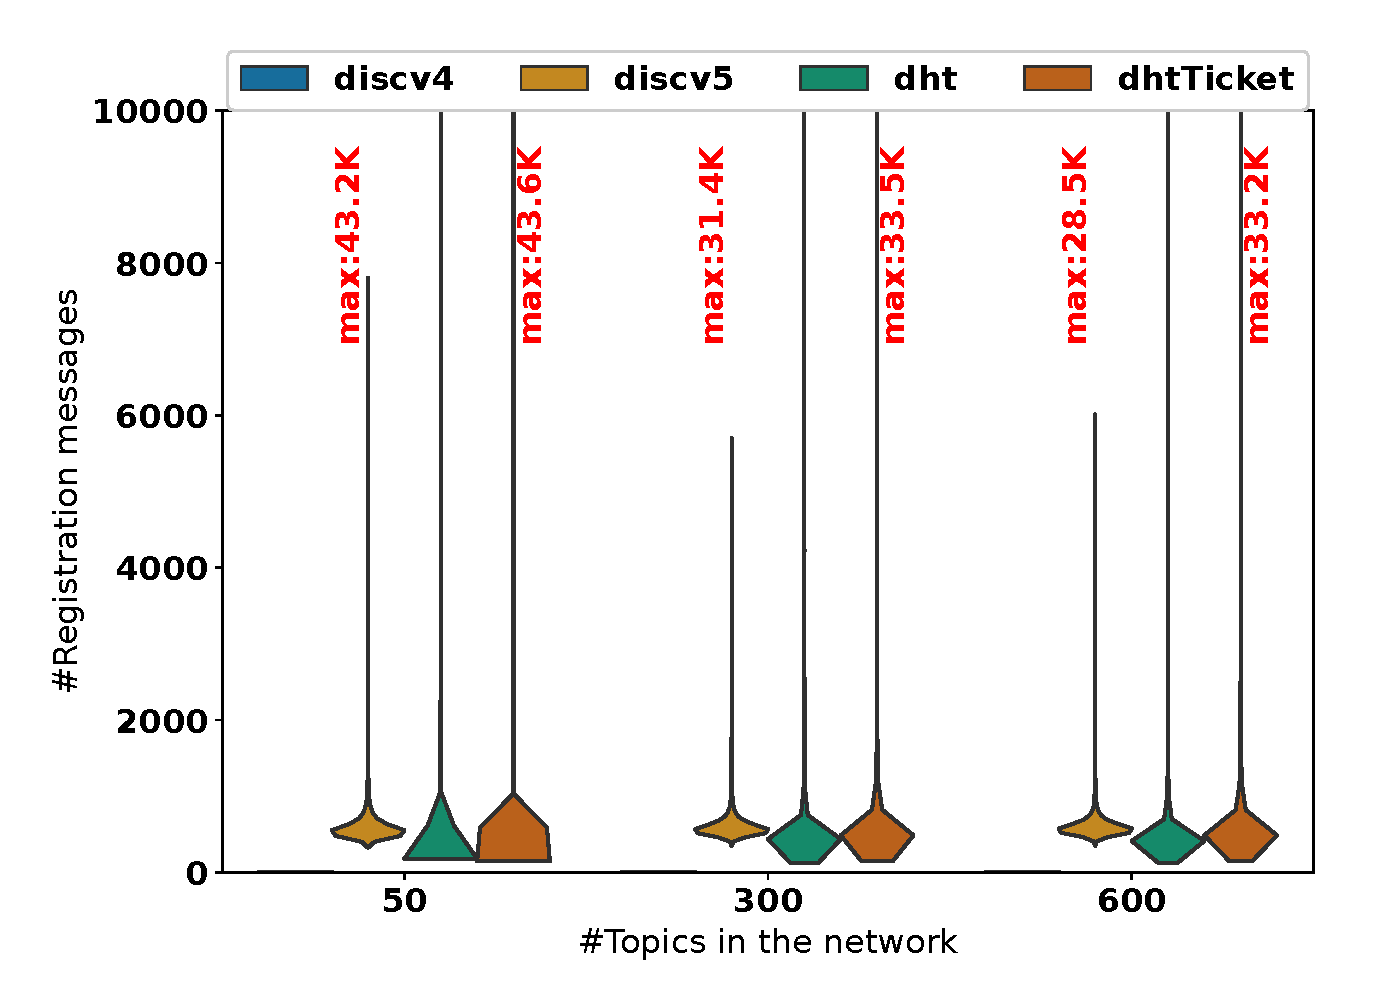
\includegraphics[width=\linewidth]{results/efficiency/violin_topic_registrationMsgs.eps}
%\caption{Y-axis: Distribution of registration related messages received by peers for varying number of topics for the simulation time.}
%\label{fig:regMsgsPerTopic}
%\end{figure}

%In~\Cref{fig:regMsgsPerTopic}~and~\Cref{fig:regMsgsPerSize},  we can observe while most of \sysname nodes receive around 500 registration messages,  with just a few receiving up to 5k messages in the worst case,  \altname solutions are more spread between 0 and 1000 received messages, but with some peaks up to 43k messages,  an order of magnitude higher than \sysname.
%This is caused by the fact that all nodes in \altname solutions try to put registrations starting by the closest nodes to the topic hash,  creating an uneven distribution  towards these nodes. 
%In \sysname, the use of \emph{advertise table} for advertisement placement provides a similar effect. 
%However this effect is diminished by the use of waiting times to regulate advertisement placement.  The increase of waiting time in the more congested nodes, causes that nodes starts more registrations in less congested nodes limiting the number of registrations placed on nodes close to topic hash.
%This effect is not seen when using \altname combined with tickets. 
%This is due to the fact that \altname is not using a \emph{advertise table} to keep track of ongoing registrations.  Because of this,  advertisers start new registrations towards the topic hash every advertisement period, even if they did not succeed in the previous attempts due to high waiting times.
%Therefore using tickets in the \altnameticket, maybe useful to increase the diversity in the \emph{advertise tables} but not for load balancing between nodes.
%
%When increasing the number of topics in the network (\Cref{fig:regMsgsPerTopic}), it is not observed an increase of registration messages for any of the different protocols. 
%However,  when increasing the number of nodes participating in the network (\Cref{fig:regMsgsPerSize}),  also registrations messages received per nodes are increased, as expected.
%But this increase is very different between \sysname and \altname protocols.
%\sr{tbc with specific values}

%\begin{figure}[!h]
%\centering
%\includegraphics[width=\linewidth]{results/split/size_registrationMsgs.eps}
%%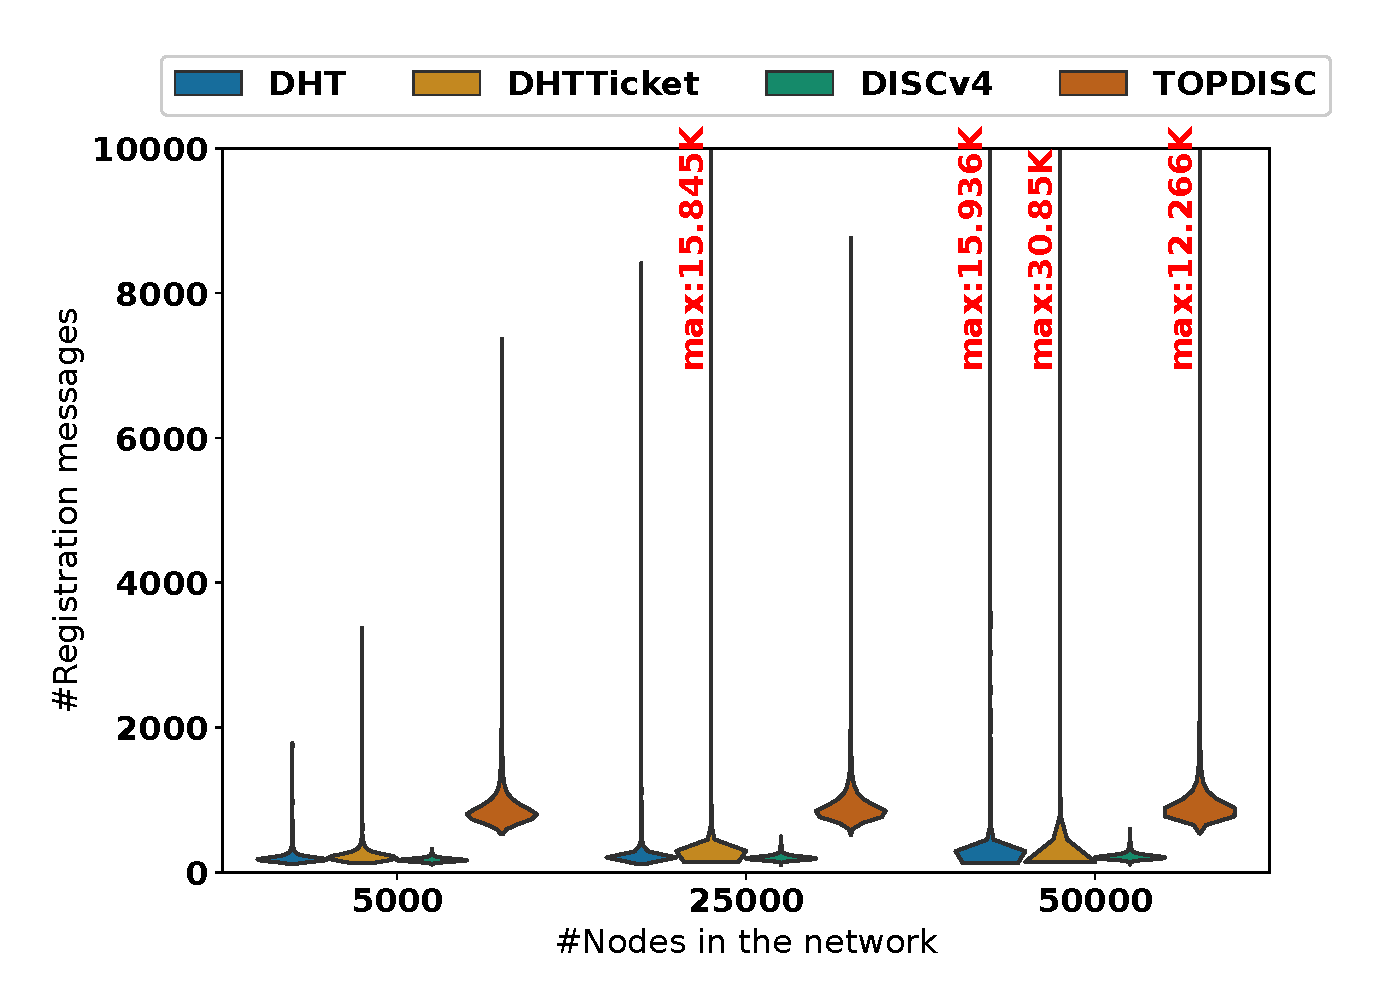
\includegraphics[width=\linewidth]{results/efficiency/violin_size_registrationMsgs.eps}
%\caption{Y-axis: Distribution of registration related messages received by peers for different network size for the simulation time.}
%\label{fig:regMsgsPerSize}
%\end{figure}
%
%\begin{figure}
%\centering
%\includegraphics[width=\linewidth]{results/split/topic_lookupMsgs.eps}
%%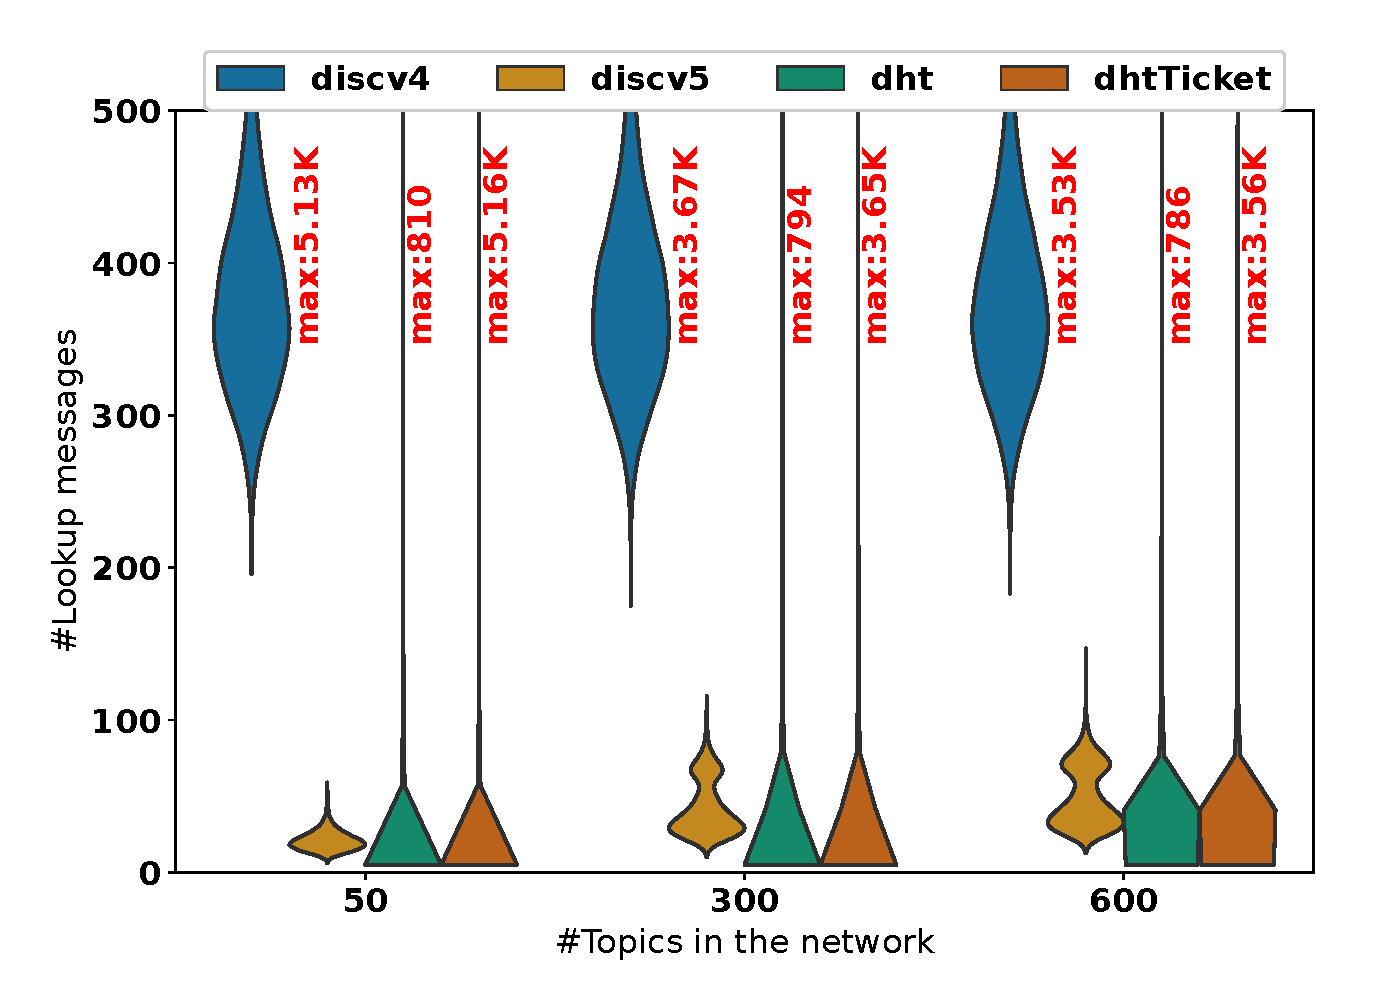
\includegraphics[width=\linewidth]{results/efficiency/violin_topic_lookupMsgs.eps}
%\caption{Y-axis: Distribution of lookup messages received by peers for varying number of topics for the simulation time.}
%\label{fig:lookupMsgPerTopic}
%\end{figure}
%
%\begin{figure}[!h]
%\centering
%\includegraphics[width=\linewidth]{results/split/size_lookupMsgs.eps}
%%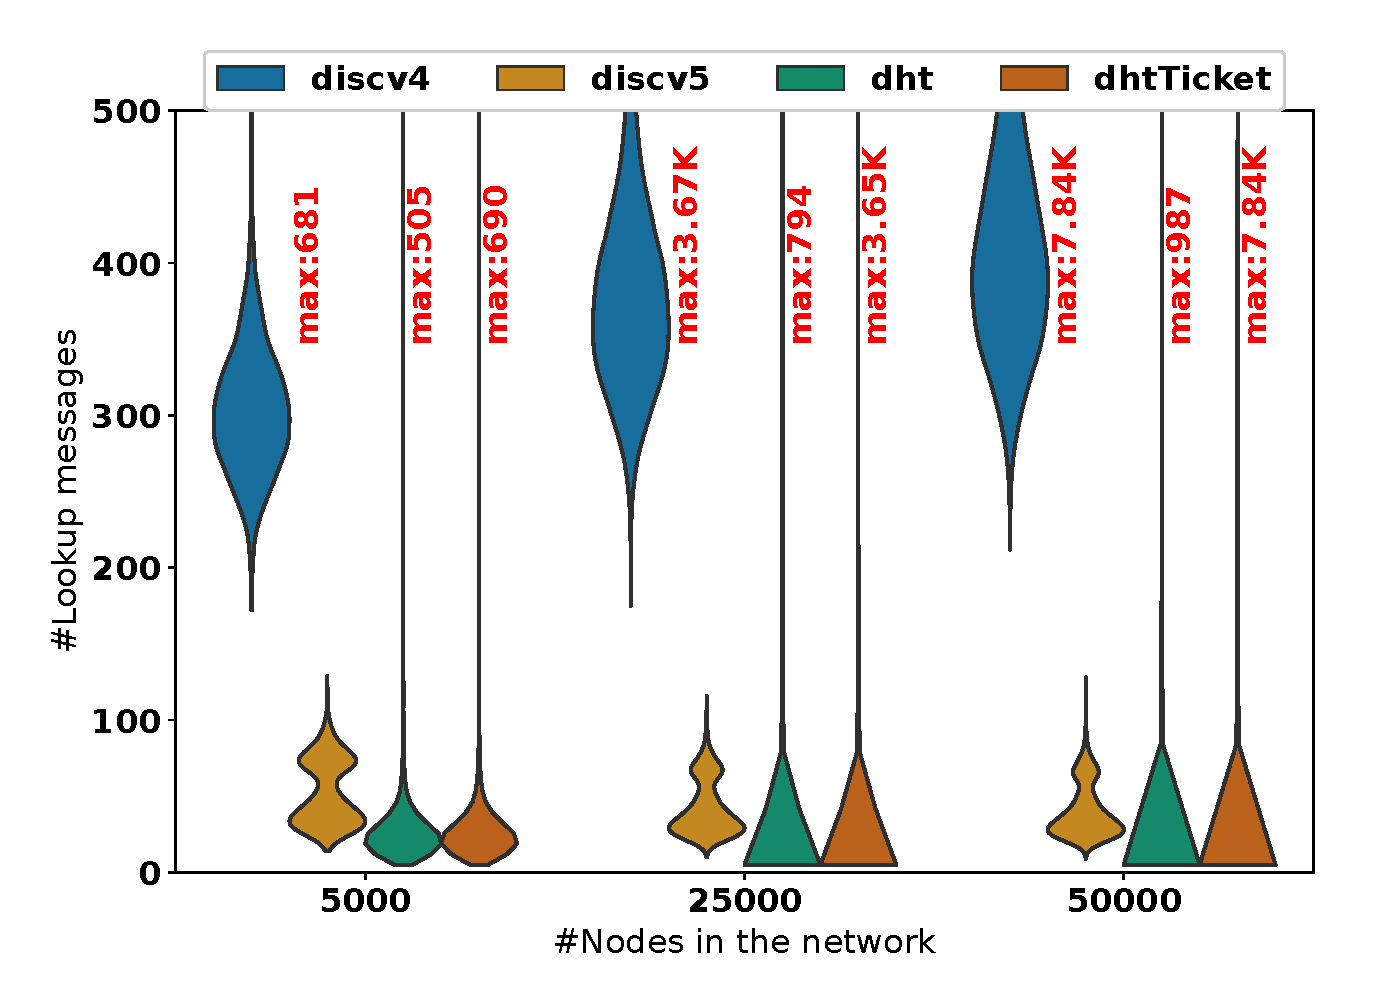
\includegraphics[width=\linewidth]{results/efficiency/violin_size_lookupMsgs.eps}
%\caption{Y-axis: Distribution of lookup messages received by peers for different network size for the simulation time.}
%\label{fig:lookupMsgPerSize}
%\end{figure}

%In~\Cref{fig:lookupMsgPerTopic}~and~\Cref{fig:lookupMsgPerSize}, we observe the number of messages related to the lookup process, \ie topic queries and replies for \sysname, \altname and \altnameticket, and kademlia find/response messages for \discv. We evaluated using  different network sizes and different number of topics in the network. 
%There is a single lookup in the simulation per node, and the $N_\textit{lookup}$ parameter used is equal to 30.  Therefore nodes stop the lookup process when found 30 different nodes in the network for the intended topic.
%In the figures we can observe there is a big different between topic-aware protocols (\sysname, \altname and \altnameticket) and \discv. 
%
%\sr{why there is an increase for \discv with the number of nodes in the simulation and not the number of topics??? shouldn't be the opposite? I guess is because even if there are topics with less nodes there is just a single lookup with the same nodes contacted}
%\sr{why the peak is bigger for DHT for 600 than 300? Is it because of topic hash ids colliding?}

\begin{figure}[!h]
\centering
\includegraphics[width=\linewidth]{results/split/size_totalMsg.eps}
%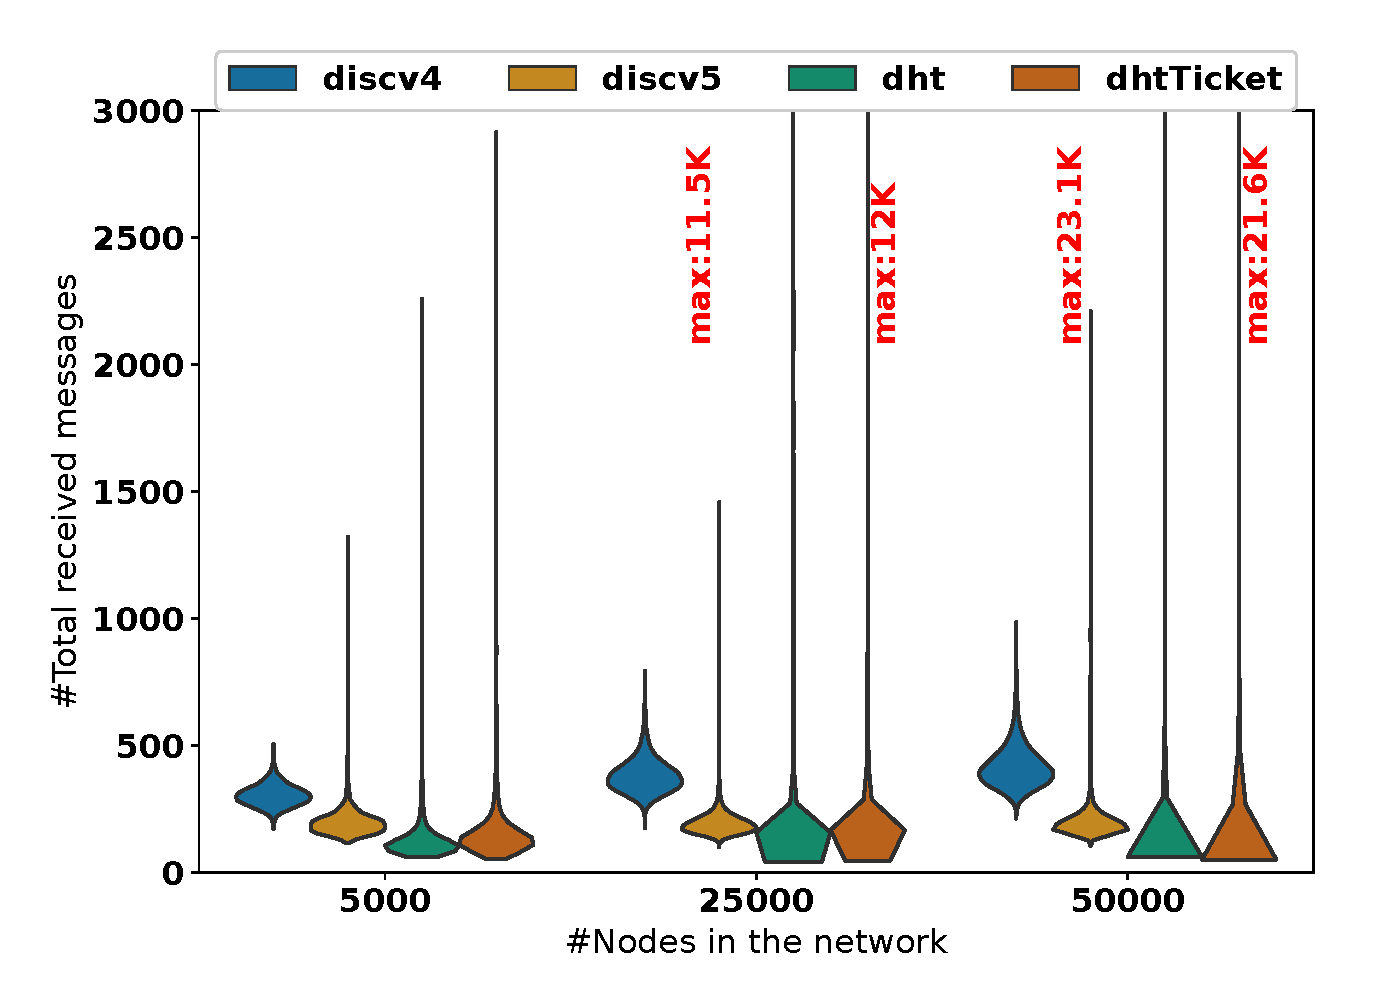
\includegraphics[width=\linewidth]{results/efficiency/violin_size_totalMsg.eps}
\caption{Y-axis: Distribution of discovery related (including registration and lookup) messages received by peers for different network size during a single advertisement period.}
\label{fig:msgsPerSize}
\end{figure}

\begin{figure}
\centering
\includegraphics[width=\linewidth]{results/split/topic_totalMsg.eps}
%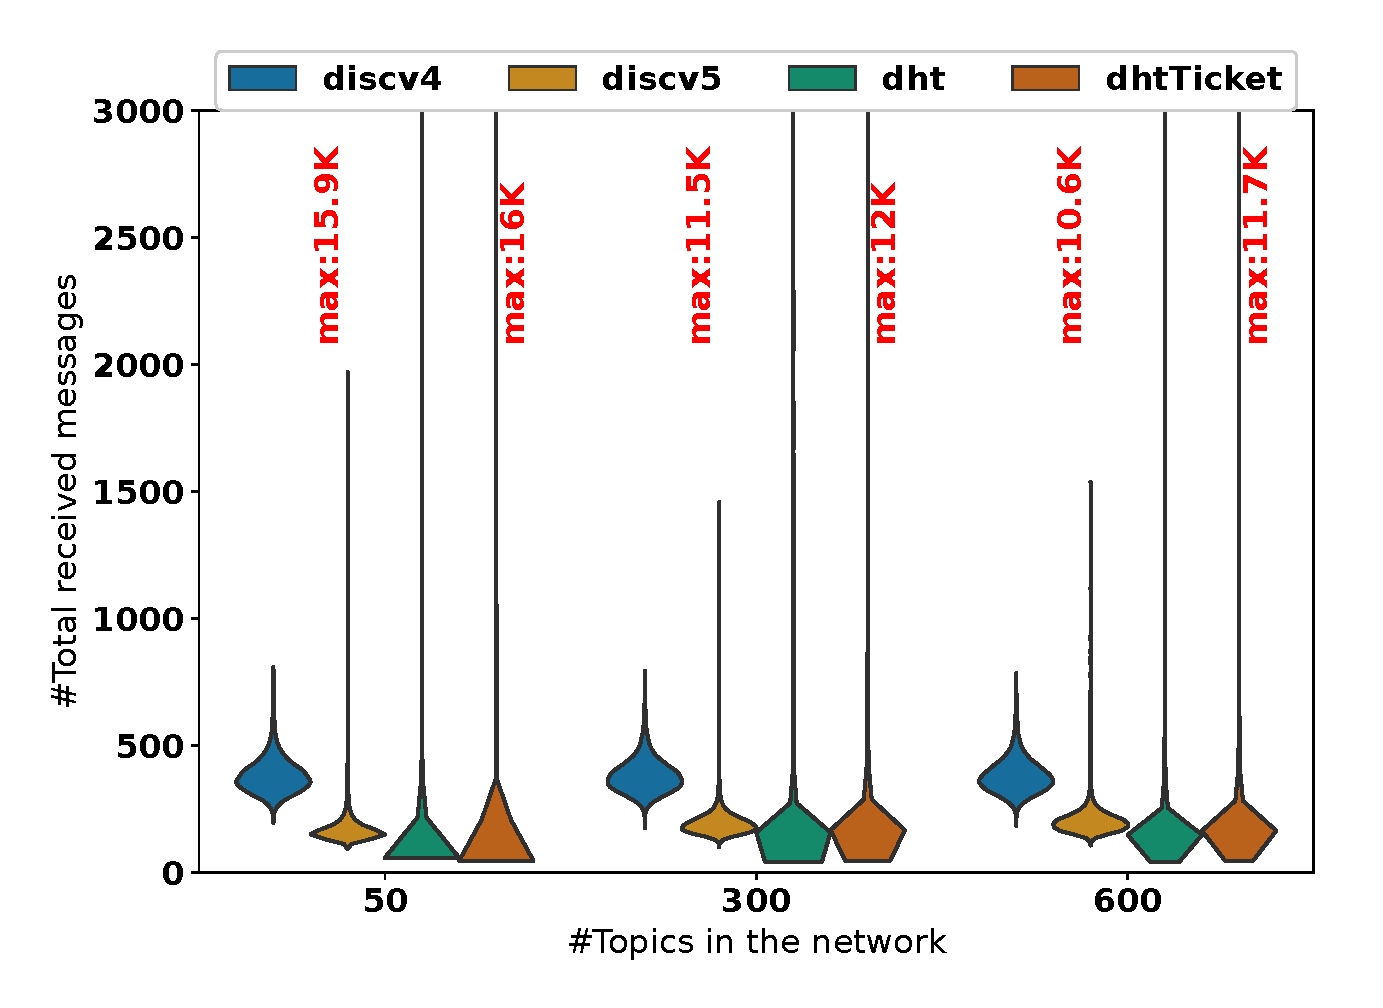
\includegraphics[width=\linewidth]{results/efficiency/violin_topic_totalMsg.eps}
\caption{Y-axis: Distribution of discovery related (including registration and lookup) messages received by peers for different number of topics during a single advertisement period.}
\label{fig:msgsPerTopic}
\end{figure}

In~\Cref{fig:msgsPerSize}~and~\Cref{fig:msgsPerTopic}, we observe the total number of messages during the simulation but normalised per advertisement period. 
Therefore in the figures, it is shown the messages related to a single lookup per node and a single registration process per node before advertisements start to expire and need to be refreshed.
This the overall overhead registered per node in the network.
We can observe that \altname protocols does not scale with the increase of nodes in the network. 
Nodes that are close to a topic hash receive most of the traffic and there is a linear increase with the number of nodes in the network. 
\discv protocol has a better distribution of the load between nodes since its behaviour is completely random. However, the average load in nodes is the highest one because of the overhead caused by not being able to find nodes for specific topics, increasing the overhead during lookup.
\sysname in comparison, provides lower overhead than the other protocols.

%%%%%%%%%%%%%%%%%%%%%%%%%%%%%%%%%%%%%%%%%%%%%%%%%%%%%%%%%%%
\subsection{Lookup performance}

\begin{figure}[!h]
\includegraphics[width=\linewidth]{results/split/topic_discovered.eps}
%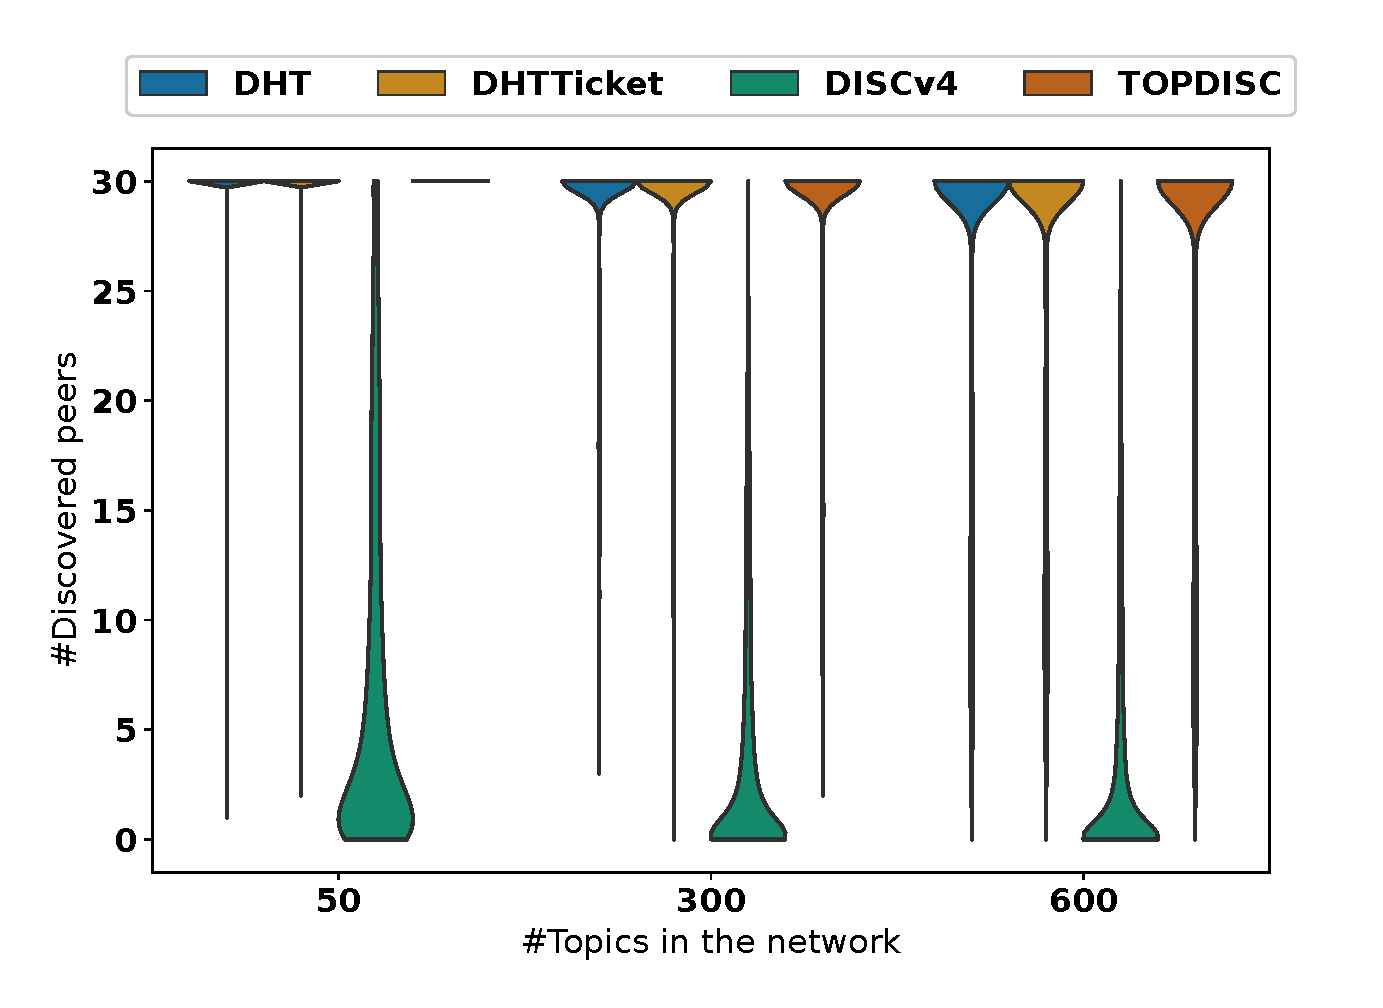
\includegraphics[width=\linewidth]{results/efficiency/violin_topic_discovered.eps}
\caption{Y-axis: Distribution of the number of peers discovered during lookup operation for different number of topics.}
\label{fig:discoveredPerTopic}
\end{figure}

\Cref{fig:discoveredPerTopic} presents the number of peers discovered during a single lookup operation with increasing number of topics in the network. The discovery becomes more difficult, as the number of topics grows.  \discv achieves a much lower number of discovered peers per operation, while \sysname and DHT-based solution efficiently discover the required amount of nodes. The rare cases where \sysname and DHT-based solution do not discover the required amount of peers are caused by small networks that consist of less than 30 nodes. 

\michal{regarding \Cref{fig:discoveredPerTopic}, it seems that for 300 and 600 topics, we discover slightly less peers on average than the DHT solutions. Why is that? Those results should be for the same topic distributions across protocols, right?}
\sergi{I think is normal and is caused by the fact that dht is going straight to nodes with most of the registrations so, specially with topics with very few nodes, they can find nodes faster, but with the tradeoff of being eclipsed very easy.}

\begin{figure}[!h]
\includegraphics[width=\linewidth]{results/split/size_discovered.eps}
%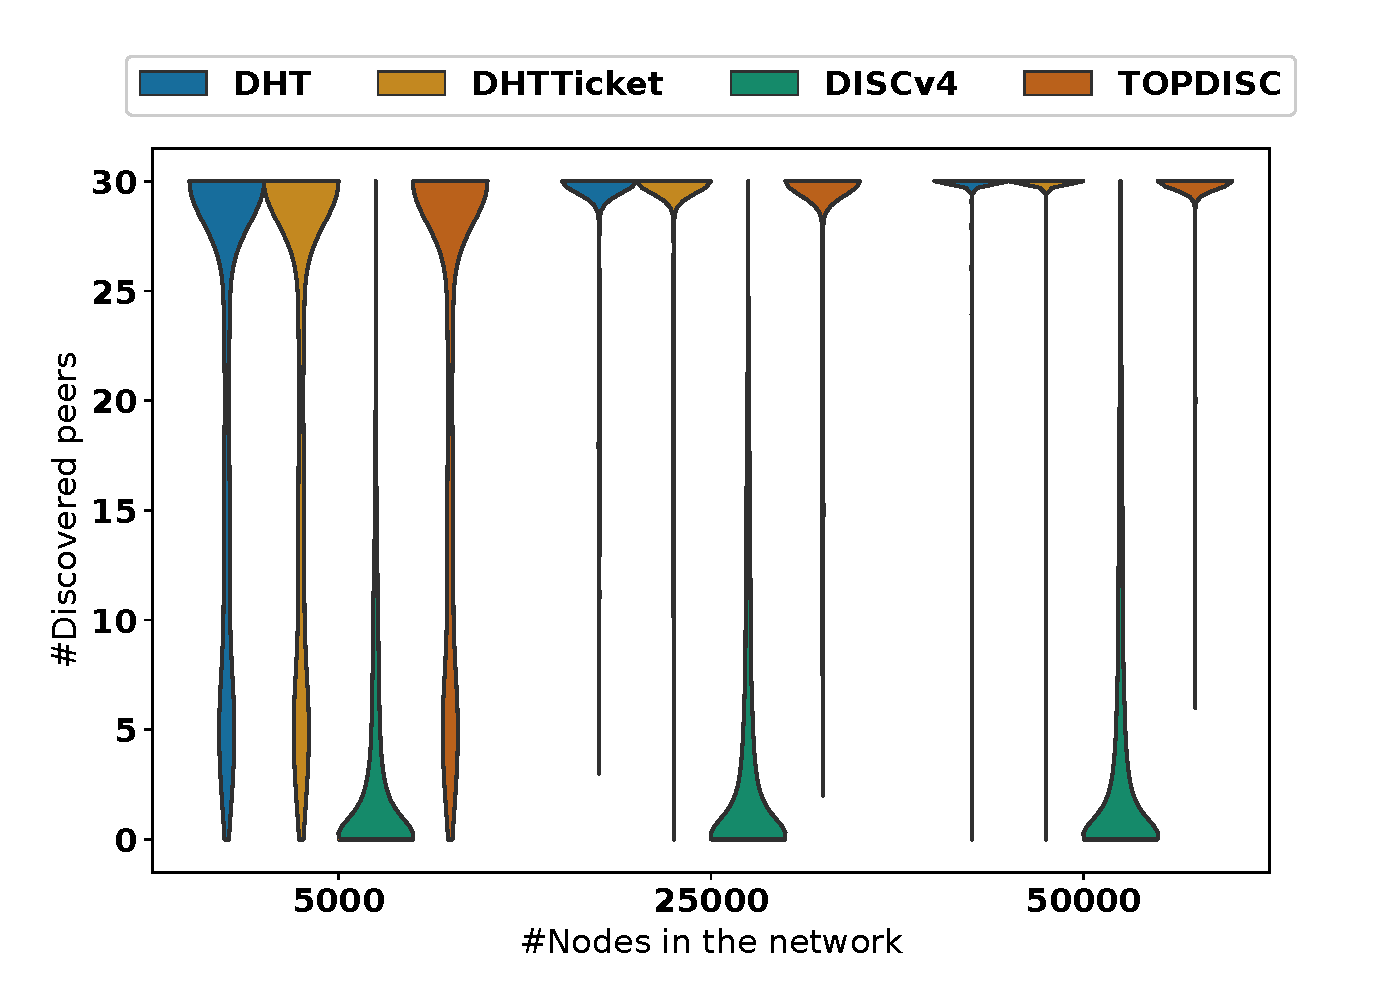
\includegraphics[width=\linewidth]{results/efficiency/violin_size_discovered.eps}
\caption{Y-axis: Distribution of the number of peers discovered during lookup operation for different network size.}
\label{fig:discoveredPerSize}
\end{figure}

\Cref{fig:discoveredPerSize} presents the number of peers discovered during a single lookup operation with increasing size of the network. With a fixed amount of topics, each application-specific network grows and for all the protocols, it is easier to find the required amount of nodes. However, discv4 suffers from poor performance for all the investigated network sizes. 

\begin{figure}
\includegraphics[width=\linewidth]{results/split/topic_wasDiscovered.eps}
%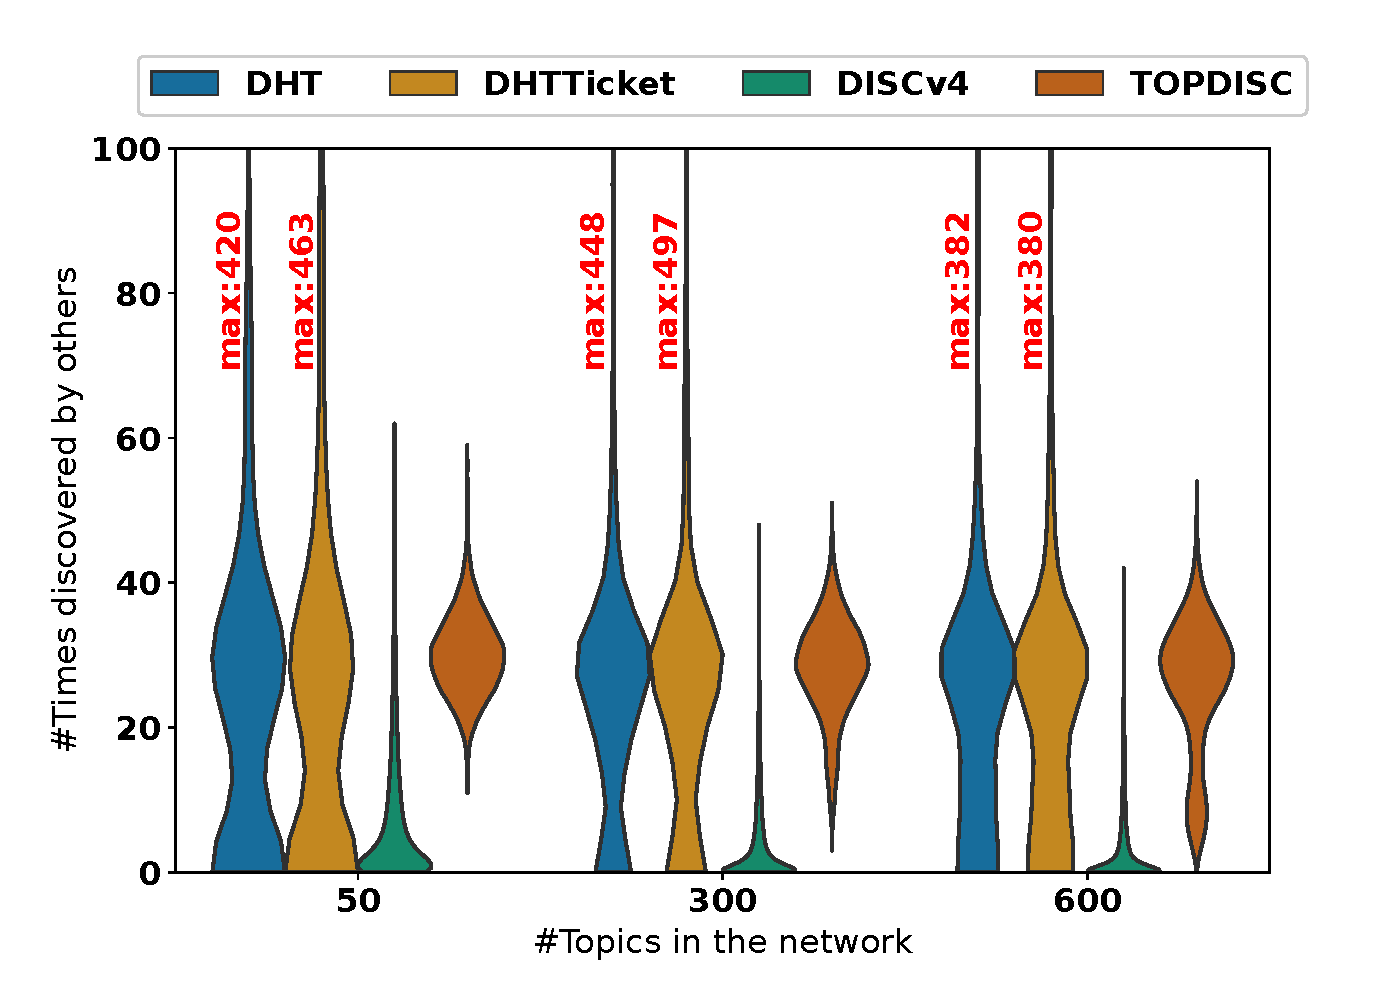
\includegraphics[width=\linewidth]{results/efficiency/violin_topic_wasDiscovered.eps}
\caption{Y-axis: Distribution of the number of times a peer is discovered by others for number of topics in the network for the simulation time.}
\label{fig:discoveredByPerTopic}
\end{figure}

\begin{figure}[!h]
\includegraphics[width=\linewidth]{results/split/size_wasDiscovered.eps}
%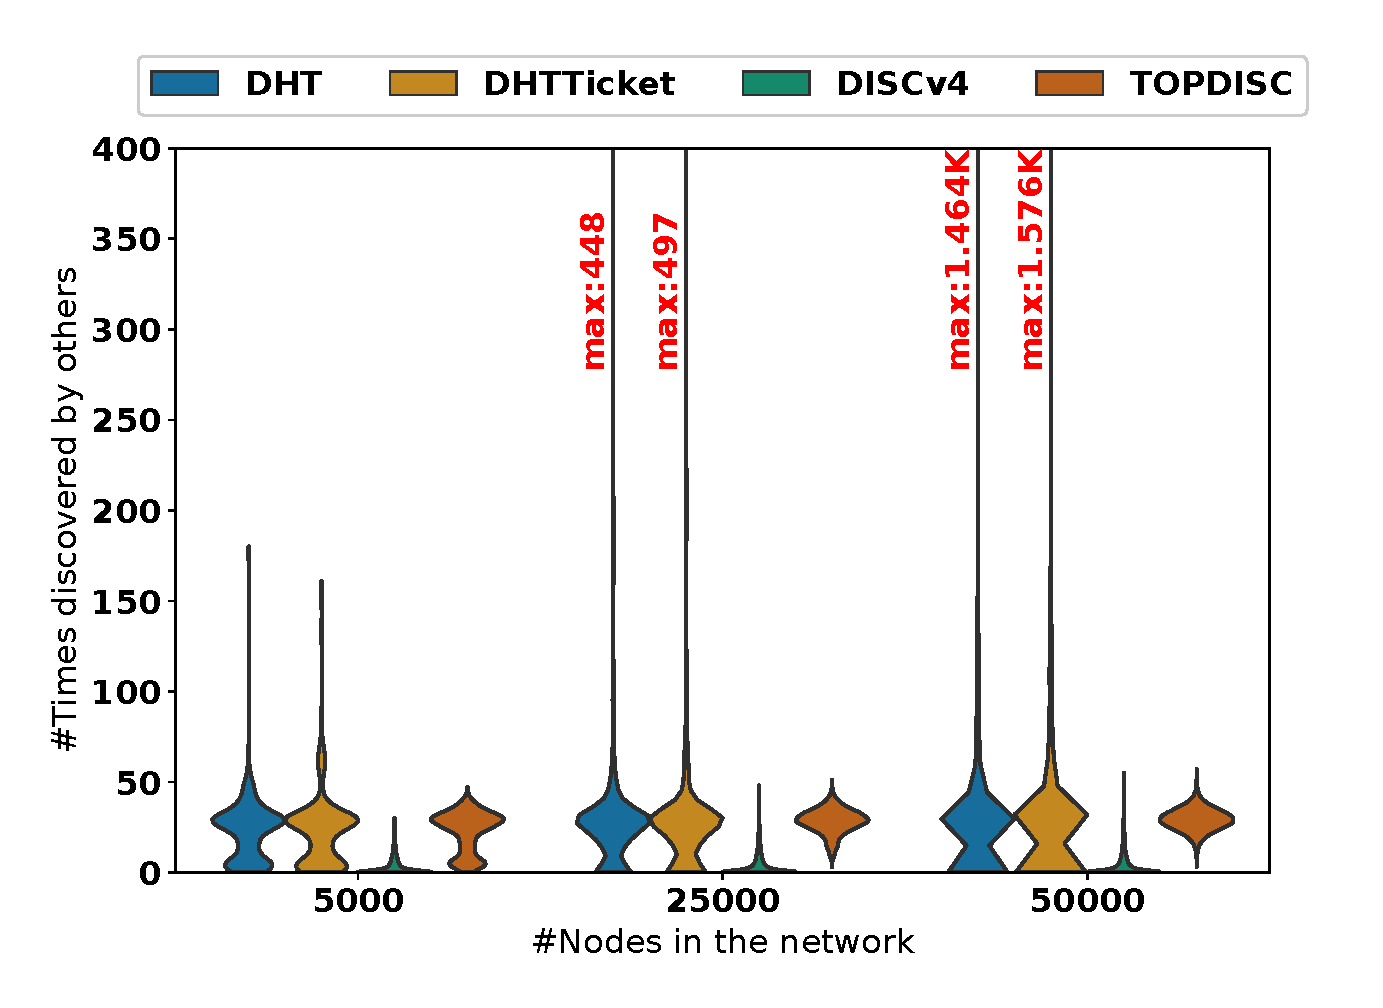
\includegraphics[width=\linewidth]{results/efficiency/violin_size_wasDiscovered.eps}
\caption{Y-axis: Distribution of the number of times a peer is discovered by others for different network size for the simulation time.}
\label{fig:efficiency_size}
\end{figure}

%\subsection{Registrations}
%
%
%\begin{figure}
%\includegraphics[width=\linewidth]{results/split/topic_regsPlaced.eps}
%%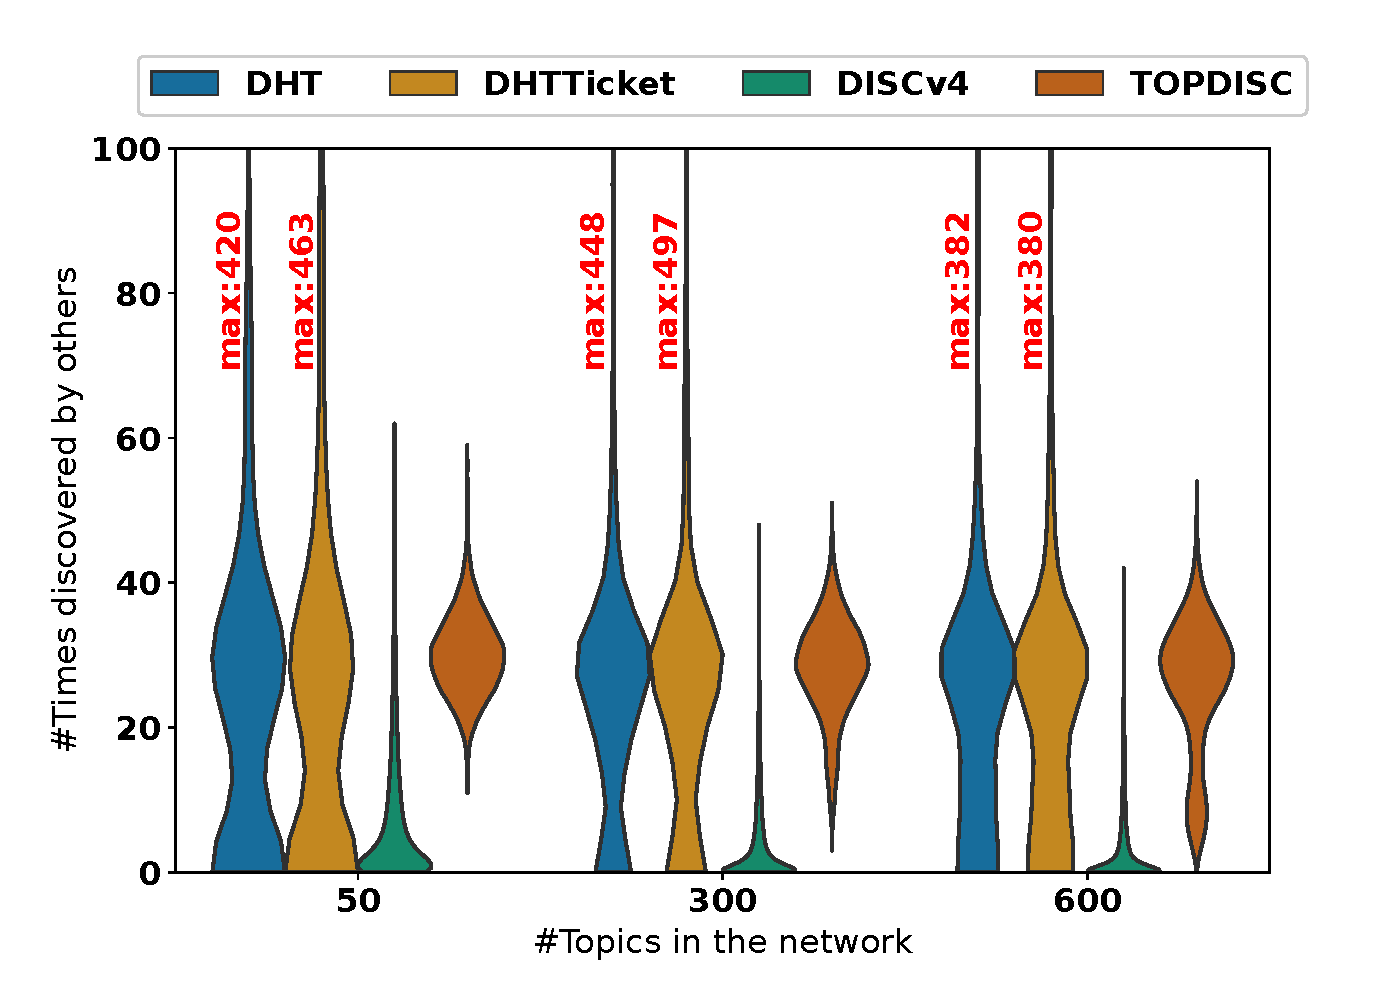
\includegraphics[width=\linewidth]{results/efficiency/violin_topic_wasDiscovered.eps}
%\caption{Y-axis: .}
%\label{fig:regsPlacedPerTopic}
%\end{figure}
%
%\begin{figure}[!h]
%\includegraphics[width=\linewidth]{results/split/size_regsPlaced.eps}
%%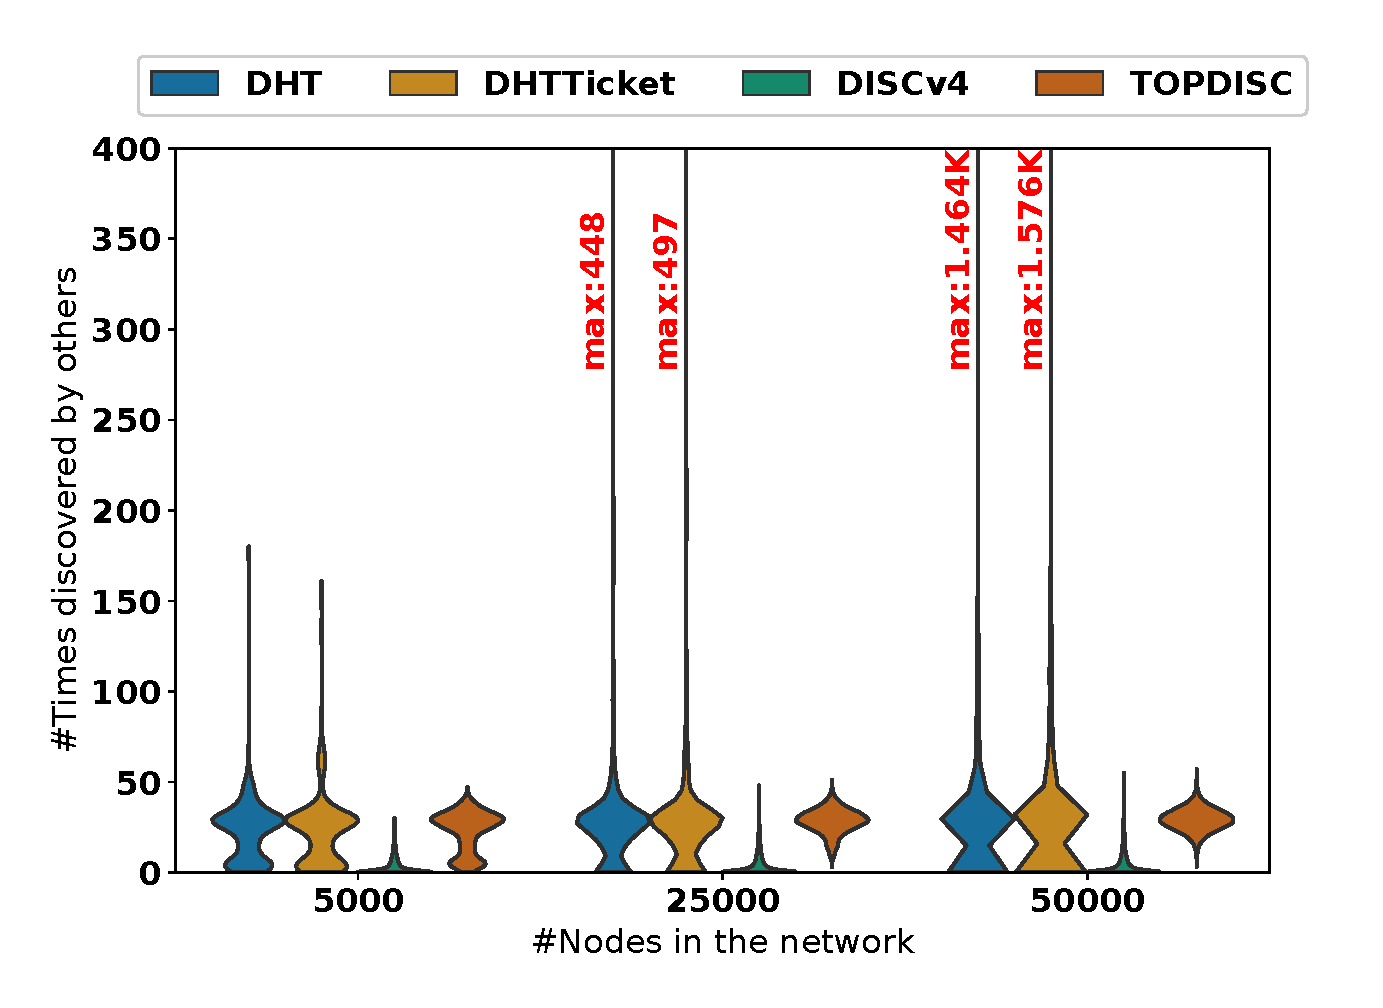
\includegraphics[width=\linewidth]{results/efficiency/violin_size_wasDiscovered.eps}
%\caption{Y-axis: .}
%\label{fig:regsPlacedPerSize}
%\end{figure}
%
%\begin{figure}
%\includegraphics[width=\linewidth]{results/split/topic_regsAccepted.eps}
%%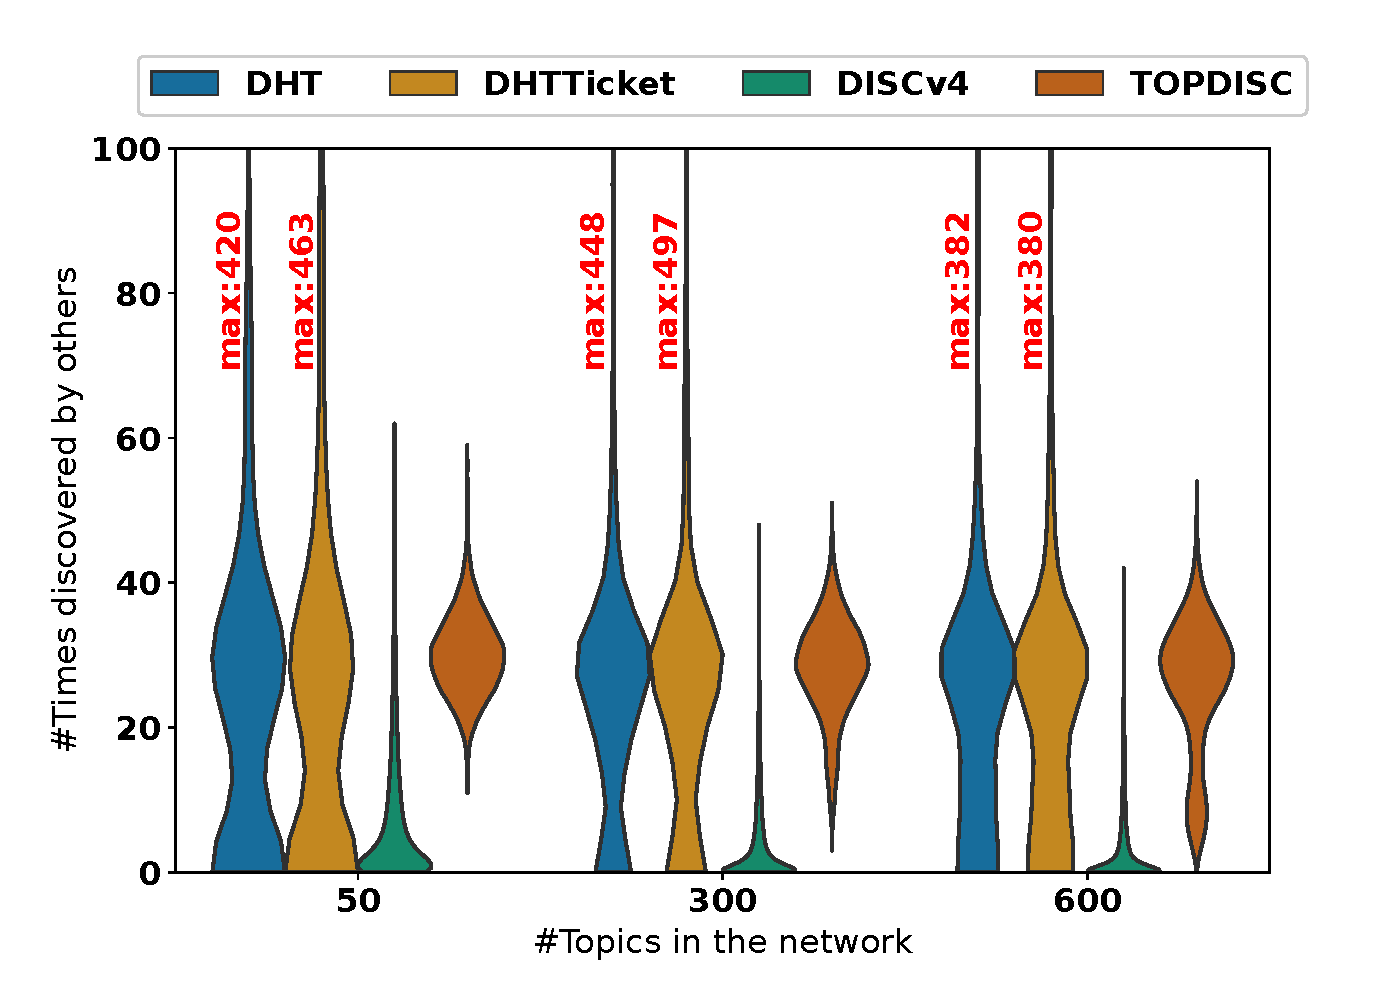
\includegraphics[width=\linewidth]{results/efficiency/violin_topic_wasDiscovered.eps}
%\caption{Y-axis: .}
%\label{fig:regsAcceptedTopic}
%\end{figure}
%
%\begin{figure}[!h]
%\includegraphics[width=\linewidth]{results/split/size_regsAccepted.eps}
%%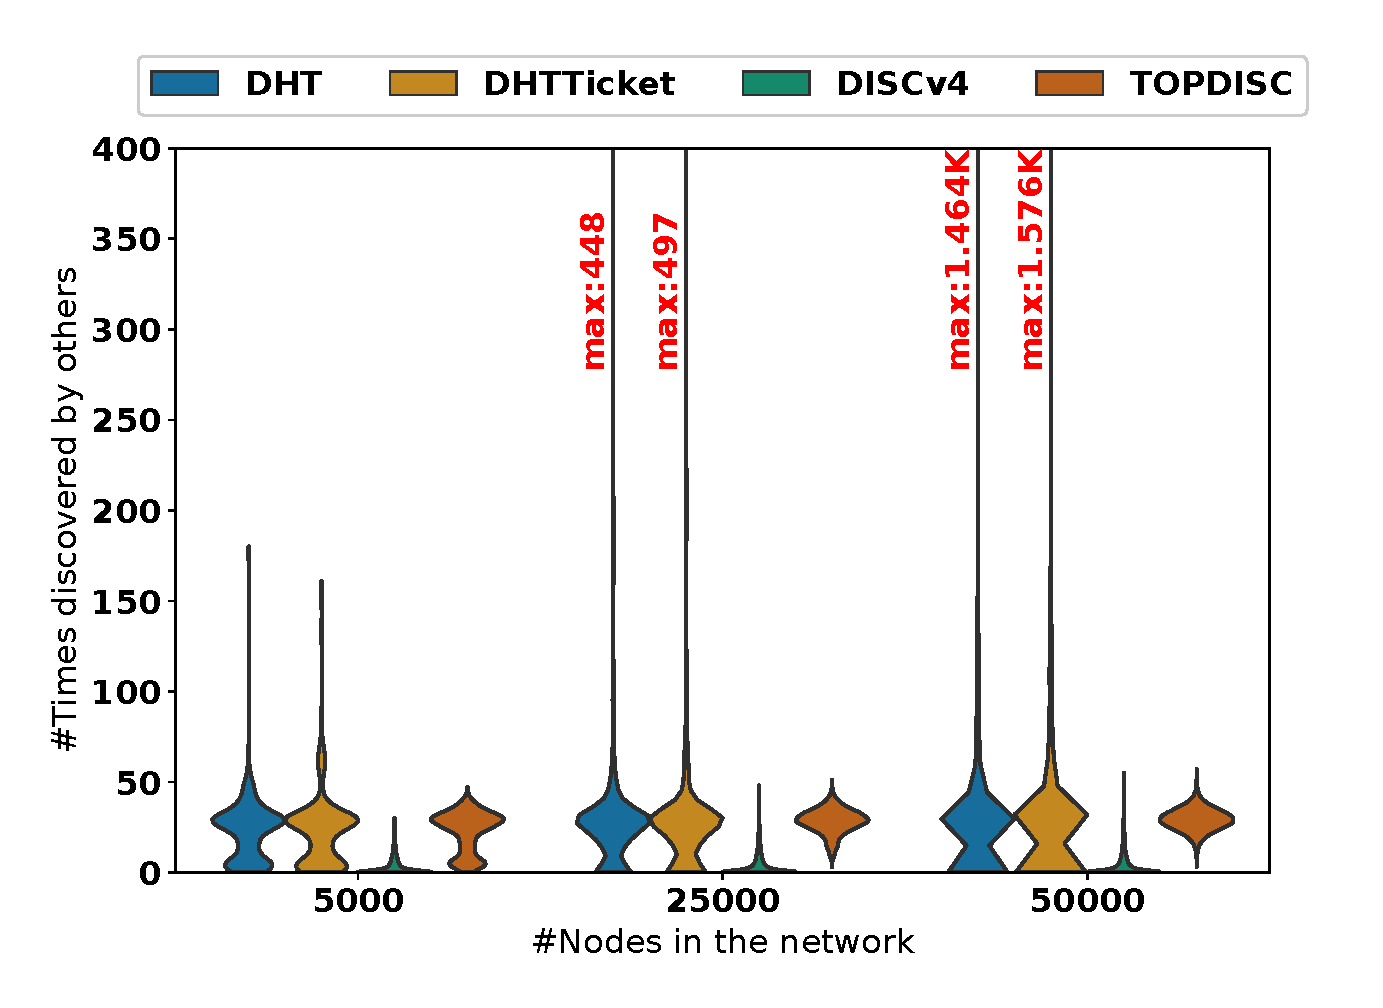
\includegraphics[width=\linewidth]{results/efficiency/violin_size_wasDiscovered.eps}
%\caption{Y-axis: .}
%\label{fig:regsAcceptedSize}
%\end{figure}

\subsection{Security}
%We evaluate \sysname resistance to two groups of malicious attacks:
%\begin{itemize}
%    \item \textbf{Eclipse Attack} - the attacker tries to make a target node discover and connect to peers under the attacker's control. The attack succeeds when all the inbound and outbound connections of the target node are established with malicious peers. 
%    \item \textbf{Denial of Service (DoS)} - the attacker tries to disturb protocol operations. The attack succeeds when service discovery is made impossible or significantly delayed for a group of benign nodes.  
%\end{itemize}
%The attacker may use a large but finite number of malicious nodes. Both attacks may target a single node or a group of nodes (\eg nodes participating in a specific application). 

%\para{Eclipse Attack}

\para{Eclipse Attack}
We implemented and evaluated \sysname resistance against a hybrid eclipse attack targeted to a specific topic,  that  tries to make a searcher node discover and connect to peers under the attacker's control.  
The attacker may be able to generate a large but finite number of Sybil nodes,  with limited network resources (\ie limited IP addresses used by the Sybil nodes pool used in the attack).
The attack succeeds when all the inbound and outbound connections of the target node are established with malicious peers.  The attack consists of the following:
\begin{itemize}
    \item \textbf{Registration spam} - the attacker targets a registrars and sends a large number of registrations requests. If successful, the attacker exhaust registrar's resources and prevent benign nodes from registering. 
%    \item \textbf{Malicious registrar} - the attacker deploys its nodes playing the role of registrars that \textit{(i)} return maximum waiting times when asked for a ticket, \textit{(ii)} return an empty set when asked about a topic. If successful, the attacker prevents benign advertisers from registering \textit{(i)} and prevents benign searchers from discovering their peers \textit{(ii)}. 
	\item \textbf{Malicious registrar} - the attacker deploys its nodes playing the role of registrars that only malicious sybils with the objective of preventing benign searchers from discovering valid peers and eclipsing all its connections.  We consider a coordinated eclipsing attack and any malicious registrar replies with a subset of the identifiers of the Sybil nodes controlled by the attacker.
\end{itemize}

We evaluated the resistance against eclipse attacks using the same default parameters used in the performance evaluation, that is 25000 nodes in the simulation and 300 topics by default, distributed using zipf function of exponent 1.0.  The simulation runs for 1 hour and there is a single lookup per node for the topic it participates.
Nodes get eclipsed when all nodes discovered during a lookup are malicious nodes controlled by the attacker, and therefore they only can connect to the attacker and get the view of the network from the attacker only. 

In the following figures we show violin plots representing the number of malicious nodes returned per lookup using different parameters for the same protocols evaluated in the performance simulations.  On top of each violin plot we specify the percentage of nodes eclipsed after a lookup (\ie percentage of lookups where all nodes returned are malicious nodes).
We evaluated the eclipse attacks targeting two specific topis, the most popular topic and a low popularity topic.
The most popular topic has 3978 nodes registering for this topic and the low popularity has only 33 nodes.
We evaluated the attacks for the most popular and least popular 


\begin{figure}[!h]
\includegraphics[width=\linewidth]{results/security/violin_idDistribution_percentageMaliciousDiscovered_t0.eps}
\caption{Y-axis: Malicious nodes discovered and percentage eclipsed nodes using uniform distributed sybil identities vs generating node ids close to topic id,   when attacking the most popular topic (3978 nodes).}
\label{fig:eclipse_distribution_t0}
\end{figure}

In Figure~\ref{fig:eclipse_distribution_t0} we show the malicious nodes discovered for all lookups for all protocols using different distribution of the identifiers of the malicious nodes,  when attacking the most popular topic (with 3978 nodes).  In the first option, the malicious nodes ids are artificially generated with a small distance to the topic hash id.  In the second option, malicious nodes identifiers are uniformly distributed.  In the figure we can observe that for \altname and \altnameticket the percentage of eclipses are superior to 80\% because most of the nodes close to topics identifiers are nodes controlled by the attacker.  
For \altname and \altnameticket, the lookup process is similar to Kademlia lookup process and,  placing all malicious nodes close the topic hash,  it makes very likely to query only malicious nodes during the process, since it only queries the closest known nodes to the topic identifier.
When attackers are uniformly distributed in the network, eclipses are reduced to close to 32.9\% and 33.7\% respectively.
Even though it is much less likely to hit malicious nodes during the lookup in this case (remember the default number of malicious are 1000 -4\% of the network-),  when hitting a malicious nodes, the nodes returned by them are used to continue the  query and it may happen it continues querying malicious nodes only during the process.
When a low popularity topic is attacked (with only 33 nodes),  as shown in Figure~\ref{fig:eclipse_distribution_t299},  for  \altname and \altnameticket the eclipses are even higher, reaching a 100\% of eclipses when placing malicious nodes close to the topic id, and reaching a 78.8\% and 90.9\% when distributing malicious nodes uniformly.  
Remember the number of attackers is 1000,  against the 33 valid nodes.

For \discv,  the number of eclipses reach is 0\% for the most popular topic when attackers are placed close to the topic hash.  When Sybil nodes are uniformly distributed the number of malicious nodes returned increases,  but to a very low 0.1\%.
This is caused by the fact that \discv does not target lookups to any specific identifier,  but completely random identifiers,  so it is very difficult for the attackers to place Sybil nodes where they will be queried.  Moreover it is difficult by the attackers to send identifiers where the lookup process will be likely to continue to,  because in the FIND node for the Ethereum DHT the lookup identifier is not disclosed,  but only the distance to it.
The number of eclipses reach 12.1.\% for the least popular topic when attackers are placed close to the topic hash.  When Sybil nodes are uniformly distributed the number of malicious nodes returned increases,  however the eclipses  reach a 78.8\%.
The resistance of \discv to Sybil attacks is obtained with the important trade-off of very low efficiency when finding nodes for specific topics, specially for low popular topics.  It is very likely that, when doing lookups using \discv for very low popular topics, no nodes are found or just a few of them.   This means when hitting a malicious node during lookup,  it is likely with a single query to a malicious node, the node querying will be eclipsed.

For \sysname, the number of eclipses are very low for the most popular topic. 
The eclipses are 0\% when Sybil nodes are placed close to topic id and 0.5\% when are uniformly distributed, with similar distribution to the malicious nodes returned compared with \discv.
However when attacking the least popular topic the eclipses increase to 78.8\% for both cases.
This is due to the very low number of valid nodes (33),  that will be more difficult to find than the attackers (1000 nodes, reusing 100 IP addresses).  
But event the high number of attackers in almost half the cases valid nodes are also found along the evil nodes.
Remember that Sybil nodes are completely valid nodes from a network discovery point of view when using different network addresses.

\begin{figure}[!h]
\includegraphics[width=\linewidth]{results/security/violin_idDistribution_percentageMaliciousDiscovered_t299.eps}
\caption{Y-axis: Malicious nodes discovered and percentage eclipsed nodes using uniform distributed sybil identities vs generating node ids close to topic id,   when attacking the low popularity topic (33 nodes).}
\label{fig:eclipse_distribution_t299}
\end{figure}

In Figure~\ref{fig:eclipse_evil_t0} we show the malicious nodes discovered for all lookups for all protocols, using different number of Sybil nodes in the network,  when attacking the most popular topic,  and in Figure~\ref{fig:eclipse_evil_t299} we show the malicious nodes discovered for the least popular topic.  In both figures attackers identifiers are generated uniformly and attackers use a pool of 100 IP addresses. 
In Figure~\ref{fig:eclipse_evil_t0}, we observe \discv is the protocol with the lowest number of eclipses and with the best distribution of malicious nodes returned during lookups.  However \sysname performs very close to \discv, having only 0.2\% of eclipses when there are 1000 attackers in the network.
\altname and \altnameticket has the worst performance,  having 47.7\% and 48.4\% of eclipses when when there are 2500 attackers.
In Figure~\ref{fig:eclipse_evil_t299}, when attacking least popular topic, we observe \sysname is the most resistant to eclipsing.
This is because it is the protocol that is able to discover more nodes with a higher diversity and is the protocol that will find easier the any of the few valid nodes in the network, and therefore it will be not eclipsed.
 
\begin{figure}[!h]
\includegraphics[width=\linewidth]{results/security/violin_percentEvil_percentageMaliciousDiscovered_t0.eps}
\caption{Y-axis: Malicious nodes discovered and percentage eclipsed nodes for different number of sybil nodes used in the attack,  when attacking the most popular topic (3978 nodes).}
\label{fig:eclipse_evil_t0}
\end{figure}

\begin{figure}[!h]
\includegraphics[width=\linewidth]{results/security/violin_percentEvil_percentageMaliciousDiscovered_t299.eps}
\caption{Y-axis: Malicious nodes discovered and percentage eclipsed nodes for different number of sybil nodes used in the attack,  when attacking the low popularity topic (33 nodes).}
\label{fig:eclipse_evil_t299}
\end{figure}


In Figure~\ref{fig:eclipse_sybil_t0} we show the malicious nodes discovered for different number of IP addresses available to the attacker,  when attacking the most popular topic,  and in Figure~\ref{fig:eclipse_sybil_t299} we show the malicious nodes discovered when attacking the least popular topic.
In this case we observe the same results than for the default values. 
\sysname is very close to \discv performance with eclipses closes to 0\% for the most popular topic, and \altname and \altnameticket is close to 33\% eclipses in all cases.
When attacking the low popularity topic,  nodes eclipsed are very similar but having a slight better performance \discv and \sysname.
There is not appreciated in the results any effect of increasing the number of IPs used by the attackers for any of the protocols.
This is caused by the fact that what is more important for the eclipses is whether you hit a malicious node during the lookup process rather than the registrations attackers are able to place in other nodes.

\begin{figure}[!h]
\includegraphics[width=\linewidth]{results/security/violin_sybilSize_percentageMaliciousDiscovered_t0.eps}
\caption{Y-axis: Malicious nodes discovered and percentage eclipsed nodes for different number IP addresses used in the attack,  when attacking the most popular topic (3978 nodes).}
\label{fig:eclipse_sybil_t0}
\end{figure}



\begin{figure}[!h]
\includegraphics[width=\linewidth]{results/security/violin_sybilSize_percentageMaliciousDiscovered_t299.eps}
\caption{Y-axis: Malicious nodes discovered and percentage eclipsed nodes for different number IP addresses used in the attack,  when attacking the least popular topic (33 nodes).}
\label{fig:eclipse_sybil_t299}
\end{figure}



%\begin{figure*}[!h]
%\centering
%\subfigure[{Y-axis: Percentage eclipsed nodes using uniform distributed sybil identities vs generating node ids close to topic id}]{
%\includegraphics[width=0.31\textwidth]{results/security/%bar_idDistribution_percentageEclipsedLookups_t0.eps}
%violin_idDistribution_percentageMaliciousDiscovered_t0.eps}
%\label{fig:distribution}
%}
%\subfigure[{Y-axis: Percentage eclipsed nodes for different number of sybil nodes in the attack.}]{
%\includegraphics[width=0.31\linewidth]{results/security/%bar_percentEvil_percentageEclipsedLookups_t0.eps}
%violin_percentEvil_percentageMaliciousDiscovered_t0.eps}
%\label{fig:percentEvil}
%}
%\subfigure[{Y-axis: Percentage eclipsed nodes for different number IP addresses used in the attack.}]{
%\includegraphics[width=0.31\linewidth]{results/security/%bar_sybilSize_percentageEclipsedLookups_t0.eps}
%violin_sybilSize_percentageMaliciousDiscovered_t0.eps}
%\label{fig:sybilsize}
%}
%\caption{Resistance against eclipse attacks when attacking most popular topic (t0)} 
%\label{fig:eclipse_attack}
%\vspace{-0.05in}
%\end{figure*}
%
%\begin{figure*}[!h]
%\centering
%\subfigure[{Y-axis: Percentage eclipsed nodes using uniform distributed sybil identities vs generating node ids close to topic id}]{
%\includegraphics[width=0.31\textwidth]{results/security/%bar_idDistribution_percentageEclipsedLookups_t299.eps}
%violin_idDistribution_percentageMaliciousDiscovered_t299.eps}
%\label{fig:distribution}
%}
%\subfigure[{Y-axis: Percentage eclipsed nodes for different number of sybil nodes in the attack.}]{
%\includegraphics[width=0.31\linewidth]{results/security/%bar_percentEvil_percentageEclipsedLookups_t299.eps}
%violin_percentEvil_percentageMaliciousDiscovered_t299.eps}
%\label{fig:percentEvil}
%}
%\subfigure[{Y-axis: Percentage eclipsed nodes for different number IP addresses used in the attack.}]{
%\includegraphics[width=0.31\linewidth]{results/security/%bar_sybilSize_percentageEclipsedLookups_t299.eps}
%violin_sybilSize_percentageMaliciousDiscovered_t299.eps}
%\label{fig:sybilsize}
%}
%\caption{Resistance against eclipse attacks when attacking least popular topic (t299)} 
%\label{fig:eclipse_attack}
%\vspace{-0.05in}
%\end{figure*}
%\begin{figure}[!h]
%
\includegraphics[width=\linewidth]{img/placeholder}
%\caption{Compare only against DHT here I guess? Y-axis a ratio of popular malicious and benign ads in the table for spam attack and topic-targeted attack within a single registrar. X-axis: to avoid showing different graphs for multiple malicious IPs/IDs/nodes we can have a fix ratio between them i.e., each 5 Sybils (or requests/s) have 1 IP and 2 ID, and increase this "attacker strength".} 
%\label{fig:security_spam}
%\end{figure}
%
%\begin{figure}[!h]
%
\includegraphics[width=\linewidth]{img/placeholder}
%\caption{Compare only against DHT here I guess? Y-axis a  time to discovery/registration (do we care about registration if lookup works?) slowdown compared to a non-attack scenario?Do we consider different placements of Sybils here (i.e., only bucket 1? Or spread evenly across all the buckets?). X-axis: to avoid showing different graphs for multiple malicious IPs/IDs/nodes we can have a fix ratio between them i.e., each 5 Sybils have 1 IP and 2 ID, and increase this "attacker strength".} 
%\label{fig:security_spam}
%\end{figure}



\iffalse
\subsection{Performance Results}
\michal{We should group the result so that they show achievement of specific goals that we described before}

%\paragraph{Ticket registrations:
In the following we detail the performance evaluation in four different subsections.  In the first we show the registration performance.  Secondly we show the traffic load and overhead of the designed mechanism.  Then we continue with the lookup and discovery performance and we finish with the security analysis.

\subsubsection{Registration  performance}

In Figure~\ref{fig:regs} we observe the average active registrations in the system per topic with different number of nodes in the simulation,  from 500 to 10000 nodes. 
We can observe nodes for all topics are able to place a substantial amount of registrations, even the less popular topics. 
As number of nodes increase in the network, we can observe the differences between registrations per topic are reduced. 
Actually, it can be observed the most popular topic (t1) is able to place less registrations than t2. 
This is caused by the fact that with more nodes trying to register for the same topic,  waiting times increase.
If the waiting time increases over the waiting time limit (in the simulations is set to 15 min),  the node cancels the registration and tries with a different nodes.
When cancellations happen it may lead to less active registrations, because it may end up with longer registration processes.
In our simulation we observe less registrations for t1 than t2  because t1 registrations waiting time go over the waiting time limit more often.

In Figure~\ref{fig:time_reg} we observe the average time necessary for a node to place a registration,  from 500 to 10000 nodes in the simulation.
We can observe that average registration time is always below 500 seconds and this is reduced for less popular topics and smaller networks. 
This figure does not include registration times for cancelled registrations.
\sergi{I think we should include failed/uncomplete registrations in the plot}

\begin{figure}[!h]
\centering
\subfigure[{Active registrations}]{
\includegraphics[width=0.225\textwidth]{img/eval/registration_origin.eps}
\label{fig:regs}
} 
\hspace{-0.25cm}
\subfigure[{Time to register}]{
\includegraphics[width=0.225\textwidth]{img/eval/avg_time_register.eps}
\label{fig:time_reg}
}
 \caption{Ticket registrations} 
\label{fig:registrations}
\vspace{-0.15in}
\end{figure}   

%\begin{figure}[h!]
%\centering
%%\epsfig{file=imgs/eval/scen5.pdf, width=0.45\textwidth}
%\includegraphics[width=0.225\textwidth]{img/eval/registration_origin.png}
%\caption{Registrations}
%\label{fig:regs}
%\vspace{-0.15in}
%\end{figure}

%\paragraph{\bf{Network load}:}
\subsubsection{Network load}

In Figure~\ref{fig:messages}~and~\ref{fig:msg_distr} we can observe the traffic load generated in the network.
In Figure~\ref{fig:messages} we observe most of the messages are ticket requests/replies, and the subsequent registration request/replies
after receiving a ticket from a node. 
This is caused by the fact that nodes are constantly registering dynamically. 
In Figure~\ref{fig:msg_distr} the messages received distribution. 
We can observe some nodes receive much more messages.
This is caused by the bucket node distribution, where nodes with identifiers close to topic hash ids receive more initial tickets requests because there are less.
However, we observe while the number of nodes in the network is increased 20 times,  the  maximum number of messages received by some nodes does not increase in the same way,  only being twice the amount when comparing 500 with 10000 nodes,  ans with increases lower than 30\% when number of nodes are doubled.
Moreover,  we can also see the number of messages received does not exceed 10 times the average value of the messages received. 

Therefore, the system is able to scale without danger of overloading some of the nodes of the network.

\begin{figure}[!h]
\centering
\subfigure[{Number of messages}]{
\includegraphics[width=0.225\textwidth]{img/eval/message_quantity.eps} 
\label{fig:messages}
} 
\hspace{-0.25cm}
\subfigure[{Message distribution}]{
\includegraphics[width=0.225\textwidth]{img/eval/messages_received.eps} %\hspace{-1.5em}%
\label{fig:msg_distr}
}
 \caption{Traffic load} 
\label{fig:traffic}
\vspace{-0.15in}
\end{figure}   

\subsubsection{Discovery and lookup performance}

%\paragraph{\bf{Discovery performance}:}

In Figure~\ref{fig:reg_disc} and \ref{fig:timedisc} we can observe how nodes are discovered within the network.
In Figure~\ref{fig:reg_disc} we observe the percentage of the nodes in the network that are discovered and how often are discovered.
Each node in the network is represented by a circle, and the size of the circle represents the relative frequency of discoveries compared with other nodes in the network.
We can observe that for all topics the percentage of nodes discovered in the network is very close to 100\%. This means almost all nodes in the network are able to be discovered by other nodes. The number of discovered nodes is not 100\% because of the existence of turbulence (there are some nodes just joined the network and there has not been enough time yet to be discovered). In case there are a low number of nodes for a specific topic (e.g. t5 with 500 nodes network) the 100\% is reached.
We can also observe Figure~\ref{fig:reg_disc} that the discovery distribution is bounded to \hl{X} times between the most discovered and the least discovered.
We observe the dots size are very regular and despite being not completely equal the differences are not substantial. 
In Figure~\ref{fig:timedisc} we observe the time between a registration is completed and the first time the registration
is returned in a lookup.
By observing this we can see how difficult is for a node to be discovered once is able to place a registration. 
We see the average time is between 20 and 10 seconds in most of the cases, except for the least popular topic t5 which is around 50\% higher. 
We also observe the deviation is bounded at around 60 seconds, with equivalent different for t5.


\begin{figure}[!h]
\centering
\subfigure[{Advertiser discovery distribution}]{
\includegraphics[width=0.225\textwidth]{img/eval/registrant_distribution.eps} 
\label{fig:reg_disc}
} 
\hspace{-0.25cm}
\subfigure[{Time between registration and first discovery}]{
\includegraphics[width=0.225\textwidth]{img/eval/min_time_discovery.eps} %\hspace{-1.5em}%
\label{fig:timedisc}
}
 \caption{Discovery performance} 
\label{fig:discovery}
\vspace{-0.15in}
\end{figure}   


In Figure~\ref{fig:hopcount} we can observe the lookup performance of \sysname compared with Discv4 for a 5000 nodes simulation.
In the plot we show the average number of nodes discovered for each hop during a lookup per topic, taking into account that Discv4 cannot do per topic lookups,  so we discard received nodes that do not support the specific service.
In the figure we observe that for t1 the discovered nodes are higher when using Discv4, since all topics support t1 and any node discovered will be a valid node. 
However, as the popularity of the topic decreases it also does the lookup performance of Discv4,  since it is very difficult to find nodes for non-popular topics without supporting per topic lookups.
In this sense,  Discv5 lookup performance also decreases the performance with non-popular topics (simply because there are less nodes in the network) however this decrease is diminished.  Between t1 and t5 the lookup performance is decrease approximately to a 1/2th for Discv5, while when using Discv4 the lookup performance decreased to a less than a 1/10th.

%TODO add lookup description including mechanisms to avoid sybils.

\begin{figure}[h!]
\centering
%\epsfig{file=imgs/eval/scen5.pdf, width=0.45\textwidth}
\includegraphics[width=0.35\textwidth]{img/eval/lookup_hopcount_discv4.png}
\caption{Lookup performance}
\label{fig:hopcount}
\vspace{-0.15in}
\end{figure}

\subsubsection{Sybil Attacks}

In the following we show the results of the performance evaluation of the discovery service under different sybil attacks.  The attacks that we evaluated in this section are of two types and are previously described in Section~\ref{sec:overview}. 
These attacks are eclipsing  and Denial-of-service (DoS) attacks.
Eclipsing attacks goal is to generate multiple fake identities within a topic to be able to eclipse existing nodes in the network.
Eclipsing a node imply all outbound and inbound connections are established to only sybil/fake nodes controlled by an attacker.
This allows the attacker to control the view of the network of the eclipsed node and can be used to co-opt a victim's mining power and use it to attack the blockchain's consensus algorithm.
DoS attacks instead is an attack meant to hamper the good performance or even to shut down the network, making it inaccessible to its intended users.  
In our case,  the goal of DoS attacks is to difficult or to block the discovery of nodes in the network and is specially important for topic with low popularity where finding all node in the network is very important.

In the implemented topic eclipsing attack,  malicious nodes are sybil nodes that cooperate in order to eclipse other valid nodes.
Malicious and valid nodes have the same amount of bandwidth resources and malicious nodes respond to topic lookup requests and find messages with only other malicious nodes.
Malicious nodes also act as evil 'advertisers' trying to place as many registrations as possible by using bigger ticket size,  with malicious registrars attack,  where evil registrars replies with only malicious nodes when receiving a topic query.

We implemented and evaluated two kind of DoS attacks.  
The first attack consists in a topic spam attack where a big number of sybil identities generated try to register for non-existing random topics.
By registering for non-existing topics,  evil nodes try to harm valid topics registrations, overflowing ad caches.
The second DoS attack consists on generating sybil identities that keep without replying when receiving valid nodes ticket requests or return very long waiting times. 
This way an attacker can try to backlog valid nodes ticket registrations.

In Figures~\ref{fig:reg_eclipse},~\ref{fig:discoverytime_eclipse}~and~\ref{fig:lookup_eclipse} we show performance results under a
topic eclipsing attack.
We compare results for topic eclipsing attacks targeted to the most popular topic (t1) and attacks targeted to the least popular topic (t5). 
In the simulation there are 2000 nodes, all of them participating in t1 and only 218 participating in t5. 
In the simulations there are an additional 20\% (400 in total) malicious nodes that target the specific topic and the number of resources used in the attack (IP addresses) vary from 1 address to 50.

\begin{figure}[!h]
\centering
\subfigure[{Active registrations eclipse attack t1 attack}]{
\includegraphics[width=0.22\textwidth]{img/eval/attack/registration_origin_t1.eps} 
\label{fig:reg_eclipse_t1}
} 
\hspace{-0.15cm}
\subfigure[{Active registrations eclipse attack t5 attack}]{
\includegraphics[width=0.22\textwidth]{img/eval/attack/registration_origin_t5.eps} %\hspace{-1.5em}%
\label{fig:reg_eclipse_t5}
}
 \caption{Active registrations under topic eclipsing attack} 
\label{fig:reg_eclipse}
\vspace{-0.15in}
\end{figure}   

In Figure~\ref{fig:reg_eclipse_t1} we observe the active registrations in the simulation per topic, for an eclipsing attack targeted to the most popular topic (t1), including active registrations of malicious nodes.
We can observe than even though the number of malicious nodes is equivalent to 20\%, the number of active registrations is lower than that. 
As expected, as the number of IP addresses used in the attack increaseas, the number of active registrations of malicious nodes also increase, since different malicious nodes with complete different IPs can not be diffierentiated from valid nodes.
For topic 5, the most vulnerable topic for being the least popular, we can observe a similar pattern of active registrations. 
However, we observe that despite malicious nodes being more (400 nodes) than valid nodes (218 nodes), active registrations of malicious nodes is kept lower than 30\% in all cases. Similarly to t1, the active registrations increase with the higher number of IPs used in the attack, since there is no way to a totally distributed attack without reusing IP addresses.


\begin{figure}[!h]
\centering
\subfigure[{Time between registration and first discovery t1 attack}]{
\includegraphics[width=0.225\textwidth]{img/eval/attack/min_time_discovery_t1.eps} 
\label{fig:discoverytime_eclipse_t1}
} 
\hspace{-0.16cm}
\subfigure[{Time between registration and first discovery t5 attack}]{
\includegraphics[width=0.225\textwidth]{img/eval/attack/min_time_discovery_t5.eps} %\hspace{-1.5em}%
\label{fig:discoverytime_eclipse_t5}
}
 \caption{Time between registration and first discovery under topic eclipsing attack} 
\label{fig:discoverytime_eclipse}
\vspace{-0.15in}
\end{figure}   

In Figure~\ref{fig:discoverytime_eclipse} we observe the average time between a node registers for a topic successfully and the node is discovered for the first time from the placed registration.
We can observe that when a topic is under attack the time required for first time discovery increases. 
This is caused by the fact that there are much more registrations in the topic caused by the attack and also that malicious nodes discovery time is higher due to the difficulty to place registrations in nodes close to the topic hash.  
We can observe that when using more IP addresses in the attack the time required to discover a node is reduced because malicious nodes are more discovered.

\begin{figure}[!h]
\centering
\subfigure[{Lookup hopcount eclipse attack t1}]{
\includegraphics[width=0.225\textwidth]{img/eval/attack/lookup_hopcount_t1.eps} 
\label{fig:lookup_eclipse_t1}
} 
\hspace{-0.16cm}
\subfigure[{Lookup hopcount eclipse attack t5}]{
\includegraphics[width=0.225\textwidth]{img/eval/attack/lookup_hopcount_t5.eps} %\hspace{-1.5em}%
\label{fig:lookup_eclipse_t5}
}
 \caption{Lookup hopcount under topic eclipsing attack} 
\label{fig:lookup_eclipse}
\vspace{-0.15in}
\end{figure}   

\sergi{redo fig14 and fig15 figures increasing font and using eps}

In Figure~\ref{fig:lookup_eclipse} we observe the lookup hopcount in the simulation per topic,  for an eclipsing attack targeted to the most popular topic (t1) and the least popular topic (t5).
We observe that despite receiving an attack targeted at a specific topic,  the lookup performance in the network is not substantially affected by the attack.

In Figure~\ref{fig:perf_spam} we observe the performance of the topic discovery system under  the topic spam attack.
\sergi{TODO: add no sybil in the graph}
In Figure~\ref{fig:active_regs_spam} we observe the average active registrations per topic increasing the number of IP addresses used by sybil identities performing the attack.  
We observe that the number of active registrations per topic are decreased under the topic spam attack being topic 1 the most affected.
However, by observing Figure~\ref{fig:hopcount_spam} we see he lookup performance is not affected and therefore there is no substantial impact of the attack in the discovery performance of the network, concluding the system is resistant to topic spam attacks.
In Figure~\ref{fig:time_register_spam} we observe the average time required for registering for a topic,  increasing the number of Ip addresses used by sybil identities performing the attack.  
We observe again it seems there is no substantial impact of the attack to the time required to register for each topic

\sergi{add spam storage used?}

\begin{figure*}[!h]
\centering
\subfigure[{Active registrations under topic spam attack}]{
\includegraphics[width=0.275\textwidth]{img/eval/attack/registration_origin_spam.png} 
\label{fig:active_regs_spam}
} 
\hspace{-0.16cm}
\subfigure[{Time to register under topic spam attack}]{
\includegraphics[width=0.275\textwidth]{img/eval/attack/avg_time_register_spam.png} %\hspace{-1.5em}%
\label{fig:time_register_spam}
}
\hspace{-0.15in}
\subfigure[{Lookup hop count topic spam attack}]{
\includegraphics[width=0.275\textwidth]{img/eval/attack/lookup_hopcount_spam.png} %\hspace{-1.5em}%
\label{fig:hopcount_spam}
}
\caption{Performance evaluation topic spam attack} 
\label{fig:perf_spam}
\vspace{-0.15in}
\end{figure*}   

In Figure~\ref{fig:perf_dos} we observe the performance of the topic discovery system under the dos attack where registrars do not respond to advertisers trying to block active registrations.
In Figure~\ref{fig:active_regs_dos} we observe the average active registrations per topic increasing the number of sybil identites from 5\% to 20\% of the nodes in the network.
We observe that the number of registrations are affected by attackers,  being more affected for very popular topics,  but less affected low popularity topics.  However in none of the cases malicious nodes are able to block the active registrations and the reduction of the performance is lower than the number of sybils used.
In Figure~\ref{fig:time_register_dos} we observe the average time required for registering for a topic,  increasing the number of sybil identites from 5\% to 20\% of the nodes in the network.
We observe in this case it seems there is no substantial impact of the attack to the time required to register for each topic
In Figure~\ref{fig:time_discovery_dos} we observe the average time between an advertiser place a registration in a registrar and another node discovers it through the registrar,  increases the number sybils again.
We also observe there is no substantial impact of the attack, concluding the system is resistant to DoS attacks.

\begin{figure*}[!h]
\centering
\subfigure[{Active registrations under DoS attack}]{
\includegraphics[width=0.275\textwidth]{img/eval/attack/registration_origin_dos.png} 
\label{fig:active_regs_dos}
} 
\hspace{-0.16cm}
\subfigure[{Time to register under DoS attack}]{
\includegraphics[width=0.275\textwidth]{img/eval/attack/avg_time_register_dos.png} %\hspace{-1.5em}%
\label{fig:time_register_dos}
}
\label{fig:discovery_dos}
\hspace{-0.15in}
\subfigure[{Time to first discovery under DoS attack}]{
\includegraphics[width=0.275\textwidth]{img/eval/attack/min_time_discovery_dos.png} %\hspace{-1.5em}%
\label{fig:time_discovery_dos}
}
\label{fig:perf_dos}
\caption{Performance evaluation no-response DoS attack} 
\vspace{-0.15in}
\end{figure*}   

\fi
%\subsection{Testbed evaluation}
%
%"Geth"~\cite{go-ethereum} performance evaluation: \hl{TBC}.


%!TEX root = ../main.tex
%=========================================================

\section{Related Work}

"Eclipsing Ethereum Peers with False Friends"~\cite{henningsen2019eclipsing} - 

"Ethereum eclipse attacks"~\cite{wust2016ethereum} - 

"Low-Resource Eclipse Attacks on Ethereum's Peer-to-Peer Network."~\cite{marcus2018low} - 

"Sybil-resistant DHT routing"~\cite{danezis2005sybil}

"Whanau: A sybil-proof distributed hash table"~\cite{lesniewski2010whanau} - 

"Sybilinfer: Detecting sybil nodes using social networks."~\cite{danezis2009sybilinfer}

"Design and evaluation of Persea, a Sybil-resistant DHT"~\cite{al2014design} - 

"Defending the sybil attack in p2p networks: Taxonomy, challenges, and a proposal for self-registration"~\cite{dinger2006defending}

"Persea: a sybil-resistant social dht"~\cite{al2013persea} - 

"Quantitative analysis of the sybil attack and effective sybil resistance in peer-to-peer systems"~\cite{jetter2010quantitative}

"A Sybil-proof one-hop DHT"~\cite{lesniewski2008sybil}

"Efficient DHT attack mitigation through peers' ID distribution"~\cite{cholez2010efficient}

"Sloppy hashing and self-organizing clusters"~\cite{freedman2003sloppy}

"S-Kademlia"~\cite{pecori2016s}

"Centralized and distributed protocols for tracker-based dynamic swarm management"~\cite{dan2012centralized}

"Supporting k-nearest service discoveries for large-scale edge computing environments"~\cite{teranishi2018supporting}

"Endorsement in Hyperledger Fabric via service discovery"~\cite{manevich2019endorsement}: allows Hyperledger Fabric client to locate available services (chaincodes) using an API since HLF version 1.2. Before the set of services (chaincodes) was hardcoded at the client and server side. Since HLF is a smaller scale private blockchain it does not require large-scale service discovery as ours and it does not need to prevent this service discovery feature from attackers.

"Decentralized identifiers for peer-to-peer service discovery"~\cite{farmer2021decentralized}: besides the service discovery feature in Ethereum itself, some applications build service discovery over Ethereum, as in this example of decentralized identifiers (there are tons of examples of web services using the blockchain to store and retrieve service representatives)~\cite{keizer2021flock}.

"Under the Hood of the Ethereum Gossip Protocol"~\cite{kiffer2021under}: a study of Ethereum gossip protocol that I did not read yet.
Ethna~\cite{wang2021ethna} seems also similar.

TERA~\cite{baldoni2007tera}: A topic-based pub/sub system based on gossip protocols and self organization. Each group of nodes registered for the same topic form a random graph in which peer sampling allows contacting random nodes and use a gossip-based dissemination protocol. A similarity to our work is that nodes advertise their dissemination group with a frequency that depends on the relative size of that group compared to other groups. This relies on gossip-based size estimation protocols. Peers in large groups advertise less often. Registrars keeps the $k$ most recent ads received. The goal is that all groups are equally represented and likely to be found through a random walk. In contrast with our work, TERA requires that all nodes be trusted for not advertising themselves too often.


%!TEX root = ../main.tex

\section{Conclusions}
\label{sec:con}
On the foundational level \sysname is the first practical, secure and efficient service discovery protocol that can be deployed in large, real-world P2P networks. It combines the efficiency of traditional DHT operations with security inherited from pseudo-random ad placement. Our novel admission protocol, while performing only simple mathematical calculations, protects against a wide range of malicious behaviours, ensures equal load distribution and promotes diversity in the network.
\sysname is scheduled for deployment in the future versions of the Ethereum platform. 
An interesting future direction is to add Sybil identities detection mechanism~\cite{cholez2010efficient} and automatically modify systems parameters to operate in a more secure, but more costly, mode (\eg by decreasing the maximum number of ads retrieved from a single registrar). 

\er{minor: some issues to fix in the biblio, such as inconsistent use of acronyms, dates, or URLs. (can do)}

{\footnotesize

\smallskip

\noindent
\textbf{Open science:} All the code will be released open source, as well as datasets and scripts allowing to reproduce our experiments.

\smallskip

\footnotesize
\noindent
\textbf{Ethics/Prevention of harm:} This research does not introduce novel potential for harm beyond mentioning what has been published by other authors in the past~\cite{marcus2018low,henningsen2019eclipsing}.
}

%%!TEX root = ../main.tex
%=========================================================

\section{Notes}
Increase the blacklisting time to sth higher than ad\_lifetime

Introd why


Discovery - state that we do a fix betad non-



\subsection{Tasks}
\begin{itemize}
    \item Write the intro
    \item Draft background
    \item List all the attacks we already considered
    \item Get past attack traces from Felix
    \item IP -> new system
    \item related work - read the remaining part + start a comparison table with our design goals
\end{itemize}
\clearpage
% ========= references =========
\bibliographystyle{plain}
\bibliography{references}
%!TEX root = ../main.tex

\appendix\label{sec:appendix}
\section{Extended Analysis}

In this appendix, we provide more details on the analysis described in Section~\ref{sec:analysis}.

\subsection{Efficiency}

Due to the admission procedure, an advertisement for a specific topic will stay only $\frac{a}{a+w}$ of the time in the table of a registrar, where $a$ is the ad lifetime in the table (when admitted) and $w$ is the average waiting time. Assuming the ``worst case'' scenario where a request achieves 0 similarity score for both the topic and its IP address, the waiting time is $w = \frac{b\cdot a}{(1 - \frac{d}{n})^{P_{occupancy}}}$, where $n$ is the table capacity and $b$ and $P_{occupancy}$ are constants defined in Section~\ref{sec:waitingTime}.
If a registrar receives $x$ such requests for that topic, the average number $d$ of ads in the table is therefore
\begin{equation}
d = \frac{x}{1 + b \cdot (1 - \frac{d}{n})^{-P_{occupancy}}} \label{eq:efficiency_d}
\end{equation}
To obtain the results shown in Figure~\ref{fig:cache_size_limit}, Equation~\ref{eq:efficiency_d} must be numerically solved for $d$. With increasing $x$, $d$ will asymptotically approach the table capacity $n$.

\subsection{Fairness}

\subsubsection{Load distribution of registration operations}

We consider two topics $A$ and $B$ that are located on the opposite sides of the DHT hashspace. The registrar closest to topic $A$ will receive ad registration requests from all $N_a$ advertisers of topic $A$. On the other hand, from the viewpoint of the $N_b$ advertisers of topic $B$, the same registrar is located in the furthest  and largest bucket, containing half of the $N$ network nodes. Therefore, the registrar will only receive, on average, $\frac{N_b\cdot K_{register}}{N/2}$ registration requests for topic $B$.

Extending Equation~\ref{eq:efficiency_d} by the topic similarity score and still assuming the ``worst case'' of complete IP address diversity, the average number of ads $d_a$ and $d_b$ for topic $A$ and $B$, respectively, in the registrar's table will be:
\begin{eqnarray}
d_a & = & \frac{N_a}{1 + (b + \frac{d_a}{d}) \cdot (1 - \frac{d}{n})^{-P_{occupancy}}}\label{eq:da_fair}\\
d_b & = & \frac{\frac{N_b\cdot K_{register}}{N/2}}{1 + (b + \frac{d_b}{d}) \cdot (1 - \frac{d}{n})^{-P_{occupancy}}}\label{eq:da_fair2}
\end{eqnarray}
where $d = d_a + d_b$. Again, this system of non-linear equations must be solved numerically for $d_a$ and $d_b$.
If topic $A$ is far more popular than topic $B$, i.e., $N_a \gg N_b$, $d_a$ will be greater than $d_b$. However, because of the topic similarity score $\frac{d_a}{d}$, the advertisements for topic $A$ will not occupy the entire table.

For a registrar the closest to topic $B$ and the furthest from topic $A$, the same equations, but with the roles of topics $A$ and $B$ switched, are obtained.

\subsubsection{Load distribution of lookup operations}

As described in Section~\ref{sec:lookup}, a searcher looking for topic $A$ will start at the furthest bucket and progress toward the closest registrar to that topic until it has received $N_{lookup}$ responses.
Let bucket~1 be the furthest bucket containing $N/2$ registrars, bucket~2 the closer bucket containing $N/4$ registrars etc. In each bucket $i$, the searcher will query $\max(K_{lookup}, \frac{N}{2^i})$ registrars.
The lookup analysis in Section~\ref{sec:analysis} requires to calculate the probability that a searcher will reach the last bucket, i.e., the closest registrar to the topic. In the following, we calculate the distribution $p_{1..t}(Resp=S)$ of the number of responses $S$ that a searcher will have received after traversing buckets 1 to $t$.

Let $p_{rr,i}(Resp=S)$ be the probability that the searcher will receive $S$ responses from a registrar $rr$ in bucket $i$. We have
\begin{eqnarray*}
p_{rr,i}(Resp=S) =\sum_{R=0}^{N_a}{} p(  & & \mbox{$rr$ received $R$ registrations}\\
                        & \wedge &  \mbox{$rr$ has $\min(S,N_{return})$ ads})
\end{eqnarray*}
where $N_{return}$ is the maximum number of responses a registrar will return. The probability that the registrar received $R$ registrations is the probability that $R$ of the $N_a$ advertisers chose the registrar. It is given by the binomial distribution:
\begin{eqnarray*}
p(\mbox{$rr$ received $R$ registrations}) = \\
\binom{N_a}{R} \left( \frac{K_{register}}{N/2^i} \right)^R \left(1 - \frac{K_{register}}{N/2^i} \right)^{N_a-R}
\end{eqnarray*}
Given $R$ registrations, the number of ads that the registrar returns can be calculated using Equation~\ref{eq:da_fair} by substituting $N_a$ with $R$. Combining both results, we can calculate the joint probability $p_{rr,i}(Resp=S)$.

Calculating the exact probability $p_{i}(Resp=S)$ that a searcher obtains $S$ responses in bucket $i$ and the probability $p_{1..t}(Resp=S)$ to obtain $S$ responses after visiting buckets 1 to $t$ is numerically intensive.
Instead, we use Monte-Carlo simulation to approximate $p_{1..t}(Resp=S)$ from $p_{rr,i}(Resp=S)$. For each bucket $1\le i \le t$, the simulation randomly draws $K_{lookup}$ samples from the distribution $p_{rr,i}(Resp=S)$, in this way simulating the querying of $K_{lookup}$ registrars per bucket. This approximation assumes that the distributon of responses for the individual registrars in a bucket are independent, which is mostly correct for large $N$. The simulation is repeated 100,000 times for the result shown in Figure~\ref{fig:fairness_lookup}.
The probability to reach the last registrar is then $p_{1..14}(Resp< N_{lookup})$.

% TODO:  explain calculation of overlaps

\subsection{Security}

The probability that a searcher is eclipsed when looking up a topic in $t$ buckets is the probability to only receive malicious ads from the contacted registrars. If the network contains $n_a$ malicious nodes, the probability that a searcher will encounter one in a bucket $i$ is $\frac{n_a}{N}$, assuming a uniform distribution of the malicious nodes.
The probability $P_i$ to receive only malicious ads from a random registrar in bucket $i$ is therefore
$$ P_{i} = \frac{n_a}{N} + (1-\frac{n_a}{N}) \cdot P_{h,i}$$
where $P_{h,i}$ is the probability that a honest registrar in bucket $i$ only returns malicious ads.
Assuming independence, the probability to only receive malicious ads from the entire bucket $i$ is $P_{i}^{K_{lookup}}$ and the probability $P_{1..t}$ to be eclipsed in all $t$ visited buckets is then
$$ P_{1..t} = \prod_{i=1}^{t} P_{i}^{K_{lookup}}$$
To calculate $P_{hi}$, we need to know the distribution of honest and malicious ads in a honest registrar.
If the registrar contains $d_h$ honest and $d_a$ malicious ads, $P_{hi}$ is the probability to randomly select only malicious ads from those $d_h+d_a$ ads, which is $\prod_{i=0}^{d_h+d_a} \frac{d_a - i}{d_h+d_a-i}$.

Calculating the distribution of $d_h$ and $d_a$ analytically is difficult due to the complexity of the waiting time calculation. Instead, we approximate $P_{hi}$ using the averages of $d_h$ and $d_a$.
On average, a registrar in bucket $i$ will receive $R_h = \frac{N_h\cdot K_{register}}{N/2^i}$ honest and $R_a = \frac{N_a\cdot K'_{register}}{N/2^i}$ malicious registration requests, where $N_h$ and $N_a$ are the number of honest and malicious registrars and $K_{register}$ and $K'_{register}$ their respective number of registration attempts.

The computation of the average $d_h$ and $d_a$ is, in principle, similar to Equations~\ref{eq:da_fair} and Equations~\ref{eq:da_fair2}. However, since an attacker will only have a limited number of IP addresses, we cannot ignore anymore the impact of the IP similarity score on the waiting time:
\begin{eqnarray}
d_h & = & \frac{R_h}{1 + (b + \frac{d_h}{d} + \mbox{IPscoreH}) \cdot (1 - \frac{d}{n})^{-P_{occupancy}}}\\
d_a & = & \frac{R_a}{1 + (b + \frac{d_a}{d} + \mbox{IPscoreA}) \cdot (1 - \frac{d}{n})^{-P_{occupancy}}}
\end{eqnarray}
where $d = d_h + d_a$. Obviously, the IP score for honest ads (IPscoreH) and malicious ads (IPscoreA) depends on the numbers of honest ads and malicious ads in the table and on the number of different IP addresses used by the advertisers. Again, these non-linear equations must be solved numerically.

In the next section, we will explain how to calculate averages for the IP scores. To simplify the understanding we will start with simple situations and complete them step by step.

\subsection{IP Score}
\textbf{Situation 1: There are already} \(\mathbf{n}\) \textbf{random
addresses in the tree. What score will a new random IP address get?}

\emph{Note: We assume completely random addresses. That means it can
happen with a certain probability that some of the random addresses are
identical.}

First level of the tree: With probability 0.5, the new address goes to the 0-branch
and the probability that branch contains more than \(\frac{n}{2}\) of
the entries is
\(P(\# 0 \geq \left\lfloor \frac{n}{2} \right\rfloor + 1)\). Also with
probability 0.5, the new address goes to the 1-branch and the
probability that branch contains more than \(\frac{n}{2}\) of the
entries is\(\ P(\# 1 \geq \left\lfloor \frac{n}{2} \right\rfloor + 1).\)
Since the binomial distribution is symmetric,
\(P\left( \# 0 \geq \left\lfloor \frac{n}{2} \right\rfloor + 1 \right) = \ P(\# 1 \geq \left\lfloor \frac{n}{2} \right\rfloor + 1)\).
The average score for the first level is:

\[\text{NatScore}_{\text{level}}(n) = \sum_{i = \left\lfloor \frac{n}{2} \right\rfloor + 1}^{n}\frac{\left( \frac{n}{i} \right)}{2^{n}} = 1 - \sum_{i = 0}^{\left\lfloor \frac{n}{2} \right\rfloor}\frac{\left( \frac{n}{i} \right)}{2^{n}}\]

%This will introduce an error if n is not an integer and multiple of two.
%The best seems to be to take the average of the two approximations:
%\[\text{NatScor}e_{\text{level}}(n) = \frac{1}{2}\left( 1 - \sum_{i = 0}^{\left\lfloor \frac{n}{2} \right\rfloor}\frac{\left( \frac{n}{i} \right)}{2^{n}} + \sum_{i = \left\lfloor \frac{n}{2} \right\rfloor + 1}^{n}\frac{\left( \frac{n}{i} \right)}{2^{n}} \right)\ \ \ \ \ \ \ \ \ \ \ \ \ \ \ \ \ \ \ \ \ \ (*)\]

We assume that the levels are independent and that we will have, on
average, \(\frac{n}{2^{i - 1}}\) entries in each subtree of level \(i\).
Using the above equation on each level gives

\[\text{Score}_{\text{random}}(n) = \frac{1}{32} \sum_{i = 1}^{32}{\text{NatScore}_{\text{level}}\left( \frac{n}{2^{i - 1}} \right)}\]

\textbf{Situation 2: There are already} \(\mathbf{n + k}\)
\textbf{addresses in the tree, however} \(\mathbf{n}\) \textbf{are
random and} \(\mathbf{k}\) \textbf{are identical. What score will a new
random IP address get?}

\emph{Note: We assume again completely random addresses. That means it can
happen with a certain probability that one of the random addresses is
identical to another random address or even to the} \(k\)
\emph{identical ones.}

Let's first define the probability that at least \(\text{b\ }\)out of
\(m\) fair coin tosses are head:

\[p(m,b) = \sum_{i = b}^{m}\frac{\left( \frac{m}{i} \right)}{2^{m}}\]

%Again, errors will be introduced if \(m\) is not a natural number.
%Better results are obtained with the approximation in equation (*) from
%situation 1.

First level (``level 0'') of the tree: With probability 0.5, the new IP address is
in the same branch as the \(k\) identical addresses. The probability
that more than half of the entries are in this branch knowing that
the $k$ identical are in this branch is:

\[p\left( n,\ \left\lfloor \frac{n + k}{2} \right\rfloor + 1 - k \right)\]

With probability 0.5, the new IP address is in the branch that only
contains random addresses. The probability to have the majority of the
entries in this branch knowing that \(k\) are definitely not in this
branch is:

\[p\left( n,\ \left\lfloor \frac{n + k}{2} \right\rfloor + 1 \right)\]

In total, the score for the first level is

\[\frac{1}{2}p\left( n,\ \left\lfloor \frac{n + k}{2} \right\rfloor + 1 - k \right) + \frac{1}{2}p\left( n,\ \left\lfloor \frac{n + k}{2} \right\rfloor + 1 \right)\]

On the second level, we have four branches, of which one contains with
certainty the \(k\) identical addresses:

\[\frac{1}{4}p\left( \frac{n}{2},\ \left\lfloor \frac{n + k}{4} \right\rfloor + 1 - k \right) + \frac{3}{4}p\left( \frac{n}{2},\ \left\lfloor \frac{n + k}{4} \right\rfloor + 1 \right)\]

And so on for the other levels. In total, the average score is:

\[
\begin{split}
\text{Score}_{\text{random}}(n,k) = \frac{1}{32} \sum_{i = 1}^{32}\left\lbrack \frac{1}{2^{i}}p\left( \frac{n}{2^{i - 1}},\ \left\lfloor \frac{n + k}{2^{i}} \right\rfloor + 1 - k \right)\right. \\
+ \left.\left( 1 - \frac{1}{2^{i}} \right) \cdot p\left( \frac{n}{2^{i - 1}},\ \left\lfloor \frac{n + k}{2^{i}} \right\rfloor + 1 \right) \right\rbrack
\end{split}
\]



\textbf{Situation 3: There are already} \(\mathbf{n + k}\)
\textbf{addresses in the tree, however} \(\mathbf{n}\) \textbf{are
random and} \(\mathbf{k}\) \textbf{are identical (also random). What
score will an IP address get that is identical to the} \(\mathbf{k}\)
\textbf{identical entries?}

The situation is similar to situation 2. However, we know that we always
stay on the branch with the \(k\) identical entries. The score is:

\[\text{Score}_{\text{identical}}(n,k) = \frac{1}{32} \sum_{i = 1}^{32}{p\left( \frac{n}{2^{i - 1}},\ \left\lfloor \frac{n + k}{2^{i}} \right\rfloor + 1 - k \right)}\]

\textbf{Situation 4: There are already}
\(\mathbf{n +}\mathbf{2}^{\mathbf{a}}\mathbf{\cdot k}\)
\textbf{addresses in the tree, however} \(\mathbf{n}\) \textbf{are
random and there are} \(\mathbf{2}^{\mathbf{a}}\) \textbf{``groups'' of}
\(\mathbf{k}\) \textbf{entries with identical addresses. Those}
\(\mathbf{2}^{\mathbf{a}}\) \textbf{addresses are distributed perfectly
over the tree. What score will a new random IP address get?}

Since the \(2^{a}\) addresses are distributed perfectly over the tree,
the new random address will see exactly \(2^{a - 1} \cdot k\) of them in
its branch at the first level, \(2^{a - 2} \cdot k\) in its branch at
the second level etc. After level \(a\), the subtrees start to behave
like in situation 2.

The score for the level \(1 \leq j \leq a\) is

\[p\left( \frac{n}{2^{j - 1}},\ \left\lfloor \frac{n + 2^{a}k}{2^{j}} \right\rfloor + 1 - 2^{a - j}k \right)\]

After level \(a\), we can apply the score of situation 2 to each
subtree:

\[
\begin{split}
{\text{IPScoreH}(n,k) = \frac{1}{32}\sum_{j = 1}^{a}{p\left( \frac{n}{2^{j - 1}},\ \left\lfloor \frac{n + 2^{a}k}{2^{j}} \right\rfloor + 1 - 2^{a - j}k \right)}
}\\
+ \frac{1}{32}\sum_{i = a + 1}^{32}\left\lbrack \frac{1}{2^{i - a}}p\left( \frac{n}{2^{i - 1}},\ \left\lfloor \frac{n + 2^{a}k}{2^{i}} \right\rfloor + 1 - k \right)+\right.\\
\left.\left( 1 - \frac{1}{2^{i - a}} \right) \cdot p\left( \frac{n}{2^{i - 1}},\ \left\lfloor \frac{n + 2^{a}k}{2^{i}} \right\rfloor + 1 \right) \right\rbrack
\end{split}
\]

\textbf{Situation 5: Like situation 4
(}\(\mathbf{n +}\mathbf{2}^{\mathbf{a}}\mathbf{\cdot k}\)
\textbf{addresses), but the new address is not random; it is one of the}
\(\mathbf{2}^{\mathbf{a}}\) \textbf{addresses.}

The score for levels 1 to \(a\) is the same as in situation 4. However,
for the levels \(> a\), the ``new'' address will always stay on a branch
that contains the \(k\) entries with the same address. For those levels,
we can use the result from situation 3.

\[
\begin{split}
\text{IPScoreA}(n,k) = \frac{1}{32} \sum_{j = 1}^{a}{p\left( \frac{n}{2^{j - 1}},\ \left\lfloor \frac{n + 2^{a}k}{2^{j}} \right\rfloor + 1 - 2^{a - j}k \right)}\\
+ \frac{1}{32} \sum_{i = a + 1}^{32}{p\left( \frac{n}{2^{i - 1}},\ \left\lfloor \frac{n + 2^{a}k}{2^{i}} \right\rfloor + 1 - k \right)}
\end{split}
\]



\end{document}
